% Use the uit-report.cls to style the document
\documentclass{uit-report}



%%%% PREAMBLE ---- here you can add packages if you need extra functionality %%%%

% Provides the \lipsum command to create "Lorem Ipsum" sample text.
\usepackage{lipsum}
\usepackage{listings,multicol}
\usepackage{varwidth} %for the varwidth minipage environment
\usepackage{pdfpages}

\setcounter{tocdepth}{1}


\usepackage{enumitem}



\begin{document}
\includepdf[pages=-]{front.pdf}
\title{Saddlebags: An Object-Oriented Parallel Computing Framework for C++}
\author{Aril Bernhard Ovesen}
\date{June 1, 2018}


% Saddlebags - A High Performance Computing Framework
%An object-oriented general-purpose parallel framework with UPC++

% Saddlebags - A distributed programming framework
% Achieving efficiency and expressiveness in data-intense and compute-intense applications with UPC++

\newpage\
\pagestyle{empty}

\mbox{}

\pagebreak
\pagenumbering{roman}
\pagestyle{firststyle}
\section*{Abstract}
\addcontentsline{toc}{chapter}{Abstract}
The volume of data generated by web services and scientific tools is increasing more rapidly than many currently available high performance computing tools are able to keep up with. There is a need for novel data abstractions and parallel computing frameworks that can handle workloads from the fields of both high performance computing and big data analysis. This thesis presents Saddlebags, a high performance computing framework built on UPC++. Saddlebags aims to achieve high performance by coupling data and computing task together to exploit data locality. Principles such as fine grained remote data access and explicit data movement is inspired by high performance computing systems, while concepts such as implicit data distribution and fault tolerance is inspired by big data systems. Saddlebags can be used on individual nodes and on compute clusters, and achieves favorable performance when compared to other modern systems on both platforms.


\newpage
\section*{Acknowledgements}
\addcontentsline{toc}{chapter}{Acknowledgements}
I wish to extend my gratitude to several people.

To Phuong H. Ha, my advisor this past year, for his input and expertise. To my good friend Tor-Arne Schmidt Nordmo, for his humor, and knowledge of basically everything. To my girlfriend Johanne, for her love and support, and for being my biggest fan. To my family: Siri, Elin and Geir, for their kindness and for making me the person I am today. And finally, thanks to everyone for believing in me.

\newpage
\tableofcontents
\pagebreak
\listoffigures
\pagebreak
\listoftables
\lstlistoflistings
\addcontentsline{toc}{chapter}{Listings}
\pagebreak

\pagestyle{empty}

\mbox{}

\newpage
\pagenumbering{arabic}
\pagestyle{secondstyle}
\setcounter{page}{1}



\chapter{Introduction}


%  State of high performance computing
%  Shared memory and message passing
%  Role of different programming models/abstractions
%  Data centric computation
%  UPC++

%Scientific applications and engineering research are undergoing a transformation
%At the end of Dennard Scaling around 2004, transistor clock frequencies could not be raised without increasing the total circuit power consumption.
%Introduced multicore, manycore and accelerator-based computing 
%The big data revolution 
%Analysis, management, and collection of large volumes of data makes up the field of data-intensive science. 

%The core of high performance computing is writing efficient and parallel applications, which is the concern of researchers from an increasing range of disciplines, from physics and chemistry to medicine and geology. While the available hardware is being steadily improved,  \cite{engineering}. 


High Performance Computing (HPC) is becoming of increased importance for scientists and researchers of a large range of disciplines, from physics and chemistry, to medicine and geology. At the very core of HPC lies the ability to write efficient and parallel software~\cite{engineering}.

The U.S Department of Energy reported in 2013 through the Advanced Scientific Computing Advisory Subcommittee that the data volumes produced by scientific experiments and simulations were increasing more rapidly than the currently available algorithms, computing systems and workflows were able to keep up with. They also reported a need for innovations in HPC and data-intensive science to address challenges with contemporary systems related to concurrency, data movement, and energy efficiency~\cite{subcommittee}.

Big data frameworks such as Apache Hadoop~\cite{hadoop}, Spark~\cite{spark} and Flink~\cite{flink} can provide simple programming interfaces for distributed algorithms, with the underlying assumption that distribution of data and computing tasks can be handled by the system without programmer input. Programmers are given functionality to access data without explicitly managing communication between nodes. These systems are often reliant on coarse grained operations, which in many cases can produce inefficient programs, and limit the programmability of a framework~\cite{husky, piccolo}. Many data analytics operations are often orders of magnitude slower when implemented in a data analytics framework like Spark, than when written with native HPC tools such as MPI~\cite{bridgingthegap}. However, with a simple programming model, support for numerous data formats, underlying fault tolerance and automated data distribution, Spark remains an attractive option for distributed big data workloads~\cite{sparkarticle}. 

As many scientific applications depend on processing high volumes of data, problems of HPC and big data analytics are converging. As the amounts of data increase, so does the importance of developing more efficient analytical tools~\cite{hpcabds}. Features from big data systems can be incorporated into HPC frameworks, to create programming models that are intuitive and higher-level, yet expressive and performant. This thesis presents Saddlebags, a framework that attempts to strike a balance between the two paradigms of parallel computing systems. Inspired by big data frameworks, Saddlebags supports automatic distribution of data and computational tasks, and removes the need for specialized communication routines based on physical location. Inspired by HPC frameworks, Saddlebags allows fine grained memory access of distributed data, and leaves data movement during computations explicit and up to the programmer.

Saddlebags takes an approach to parallelism similar to graph frameworks \cite{pregel, giraph} that distribute data in vertices, and allow computational tasks to be executed within the context of each individual vertex. Saddlebags aims to support various classifications of workloads, including graph computation, and provides a vertex-like abstraction called Items. Applications are built with Saddlebags by extending an \texttt{Item} class, and creating custom item objects that contain data and computational tasks.

Saddlebags is implemented in C++. It uses parallelization and communication implementations from UPC++, a Partitioned Global Address Space library. With UPC++, a program has a static number of threads, each of which is given the affinity of a unique private memory segment. While data can be shared across segments, a memory segment is mainly accessed by the thread it has affinity to. Saddlebags applications can be used either on a single node or across multiple nodes within a compute cluster, using Ethernet or InfiniBand for network communication.



%while still allowing fine grained memory access, 


%Advantageous programming models from big data systems can be incorporated into 


%By incorporating concepts of simple programming models from big data systems, into HPC frameworks typically known for complex, we can develop tools that can solve problems that depend on both big data processing and performant computation.

%As the importance of advanced big data analytics

%Highly performant communication or computation a


%Designing efficient, yet intuitive programming models for distributed computing and data analytics seems to .
\newpage
\section{Contributions}
In brief, we make the following contributions

\begin{itemize}
	\item We design and implement Saddlebags, a High Performance Computing framework and programming model that borrows features from several other HPC frameworks and big data systems, with the aim of supporting workloads of different classifications.
	\item With the implementation of this framework, we use the UPC++ PGAS library as a communication layer for more advanced abstractions. To our knowledge, this is the first HPC framework built with UPC++.
	\item We implement several different protocols for communication between concurrent partitions, and evaluate their performance characteristics.
\end{itemize}






%A framework for implementing distributed algorithms and applications, created in and for C++, using UPC++, a library that provides PGAS mechanisms for communication. The framework provides an alternate programming model for distributed algorithms, in which a computational task, its data and its communication routines, is represented as a single object. 

% Distribution based on 


\section{Outline}
This thesis is organized as follows. Chapter 2 presents background knowledge required to understand the rest of the thesis, including a summary of related work. Chapter 3 presents principles of Partitioned Global Address Space programming, and provides an overview of the UPC++ library. Chapter 4 describes the design of Saddlebags. Chapter 5 describes details of the implementation. Chapter 6 then covers an experimental evaluation of the system. Chapter 7 discusses topics related to Saddlebags that has not been covered in other sections, and describes potential future work and improvements to the system. Chapter 8 concludes the thesis.

\newpage
\mbox{} \pagebreak
\chapter{Background}
This chapter will present an overview of the background behind this thesis. The purpose of this is to provide a technical and historical context of the work that will be presented in the following chapters. A key concept that is referenced throughout the thesis is High Performance Computing (HPC). This term refers to the technical field of working with supercomputers to solve complex computational problems. This involves the development of parallel algorithms, distributed systems and computing platforms, to meet a demand for high processing speeds~\cite{hpc_def}.

%  History + State of distributed computing / high performance computing
%  Message passing vs PGAS
%  Data intensive computing
%  Coupling of Data and processing task -> computation close to data
%  benefits of Abstractions + introduce data/task coupling as a potential 
%  Object oriented high performance computing: object contains data AND task
%  Distributed objects
%  
\section{High Performance Computing}
%The field of high performance computing has experienced two major disruptions during the 21st century.

Software performance gains from increased frequency in single processing units reached its limits many years ago, and multi-core systems has been prominent in personal computing since. Up until the early 2000s, the speed at which computers could execute sequential programs would steadily increase as clock speed and semiconductor fabrication improved \cite{sutter_larus_2005}. Heat dissipation and energy consumption caused development of the maximum achievable CPU frequency to stall, effectively freezing the number of tasks that could be completed within a certain time frame on a single processing unit \cite{diaz_munoz-caro_nino_2012}. The answers to these problems were multi-core and many-core systems, which bypasses the aforementioned performance wall by utilizing several processing~units.


Within the field of High Performance Computing, multi-processor systems were not a novelty. Using networks of workstation computers for parallel computation was already an attractive alternative to traditional supercomputers, partly because new processor technology could easily be incorporated without replacing the entire system \cite{wilkinson_allen_2005}. While the field of parallel programming was relevant in high-end scientific applications before halt in clock speed development and the following concurrency revolution, homogeneous distributed systems now dominate the field of HPC. The largest and fastest supercomputers in the world today contain millions of processor cores \cite{top500}.


Multi-core and many-core architectures achieve parallelism through explicit task distribution and scheduling, managed by the programmer. Exploiting parallelism is often an application-specific issue, and can pose several challenges. In the fields of distributed- and high performance-computing, aiming for scalability further increases the complexity of the programming task. Several programming models have been devised to support development of distributed, parallel applications, and the current leading models can be clustered into different language paradigms: \emph{shared memory }and \emph{message passing} \cite{pgas_languages}. On top of these communication models, abstractions can be applied to hide complexity from the programmer in order to reduce development time and ease the debugging process. 

\section{Programming models}

There exists a perception that abstractions carry an inherent performance penalty, but abstractions can also be powerful tools within HPC \cite{mccandless_lumsdaine_1997}. For example, computing at a large scale can introduce issues relating to handling large amounts of data, scaling to a large or arbitrary number of computation nodes, or developing algorithms that utilizes communication routines and synchronization.

Identifying common patterns in different problems allows for development of frameworks and libraries that are optimized to handle classes of problems matching the same patterns. For example, the MapReduce framework hides significant programming overhead of problems that can be expressed within semantics provided by the framework and the programming model it represents. In its most primitive, data is supplied to the \emph{Map} function and a function to execute on the data is supplied to the \emph{Reduce} function. The MapReduce programming model is designed for algorithms and problems that can be expressed using these two functions, and the MapReduce framework is implemented to provide functionality that can be applied generally to problems within that programming model.

In addition to implementing communication routines and data distribution logic, a framework can supply scalability and fault tolerance, due to the information about the application that is implied by the programming model it is utilizing. Other examples of systems specialized in specific programming models include Dryad \cite{dryad}, which models an application's data flow into directed acyclic graphs.

\section{Data intensive computing}
% asdf HPC vs big data
Many scientific fields are driven by collection and analysis of large amounts of data, and the workflows of many scientific communities based on either data analysis or computing tasks have in recent years converged towards solving similar problems \cite{bigdataconvergence}. Terms like \emph{data deluge} and \emph{Big Data revolution} are used to describe the volume of data generated by modern scientific tools and web applications. For example, large data volumes are generated by instruments such as high resolution microscopes \cite{microscopy} and gene sequencers \cite{mapreduce_locality}, or online enterprises such as Google, Facebook and Amazon. In fields of research, applications can use workflows that interweave simulations and data analysis, or that utilize both data generation and data consumption. 

Historically, data intensive sciences and computational science has been considered separate scientific fields, which has required different classes of applications and tools \cite{Hey2009JimGO}. It has also been proposed that data analysis and intensive computation can be considered different steps in a generalized scientific process, in which data analysis is a fundamental observational step, and computation is used to deduct conclusions from theories built on the available data \cite{honavar2016accelerating}. Such an understanding of a contemporary scientific method would incur that the field of computer science, traditionally aimed at solving computational problems given a problem and a set of input data, would be expanded to data gathering and exploration as well, not as an end goal, but as a step in a larger process.

A view of unified challenges in data intensive computing and HPC can formulate opportunities that benefit both fields. This can apply for two classes of workloads. Firstly, problems that require interweaved tasks of data analysis and computations will require unified application ecosystems and platforms. Secondly, problems that are defined with discrete steps of either data consumption and data analysis can benefit from the improvement in technology from both fields and their applications separately. In practice, the use of multiple platforms for solving a single pipelined problem can incur performance penalties due to differences in data structure and problem formulations~\cite{husky}. This penalty may grow larger as data volumes increase.

The convergence of workloads in HPC and big data analysis has caused some to conclude that there is a need for new applications, platforms, or data abstractions that can be applied to problems of both classes. Work has gone into merging existing big data frameworks with HPC technology~\cite{bridgingthegap, gittens2016matrix}, and devising new abstractions and data structures \cite{yang2017best}. Detailed descriptions of problems that benefit from merging workflows from big data analytics and HPC are given in \cite{subcommittee} and \cite{bigdataconvergence}.

\section{Related work} \label{section:relatedwork}
Presentations of several modern HPC frameworks and big data systems follow. These systems are described here because they in-part make up the current state of the art HPC techniques and programming models. The conflicting principles of compute-oriented and data-oriented computation are exemplified in the features of the systems that are in use today.

\subsection{Pregel}
Pregel \cite{pregel} is a system for distributed graph processing, first presented in 2010. Pregel was designed to scalably process large graphs created by web services. The workflow of Pregel involves distributing the vertices of a graph across nodes in a cluster, and performing independent computational tasks on each vertex. These tasks are performed iteratively, meaning that individual vertices may execute tasks in parallel, but the beginning and end of an iteration is synchronous. In Pregel, these iterations are called \emph{supersteps}. The execution model of supersteps is equivalent to a Bulk Synchronous Parallel execution model, from which Pregel claims inspiration. 

Vertices are distributed across a cluster by partitioning the graph into subgraphs, consisting of vertices and edges, each of which is assigned a compute node. Each vertex in the graph will execute some user-defined work task, and may as a result of this task vote to end the graph processing. The system will execute supersteps until every vertex is in agreement of ending the computation. Vertices can communicate by sending their value to other vertices, and \emph{aggregators} provide a form of communication through global monitoring of all data. Messages that are received in one superstep is available in computation during the next superstep.

A node is classified as either the master or a worker. A worker contains vertices, and executes the computational tasks associated with them. A master coordinates the activity of the workers, including handling data input, output, and global barrier synchronization. The master is also responsible for detecting faults in the active workers, initiating fault recovery mechanisms that are implemented through checkpointing.

Pregel claims better performance than MapReduce-based workflows through passing messages directly to the nodes containing relevant vertices. This is in contrast to expressing a graph as a chain of application states, where the entire graph must be re-created and re-distributed for each iteration.

\subsection{Spark}
Apache Spark \cite{spark} is a framework for big data applications, initially released in 2014. Spark aims to provide a unified programming model for different distributed workloads that handles large amounts of data. Spark is based around Resilient Distributed Datasets (RDDs), an abstract data type that implicitly distributes data across nodes and provides fault tolerance through re-creation of the data on faulty nodes. Spark provides an extension of the MapReduce model, that aims to support iterative and streaming operations more efficiently through data-sharing across multiple stages of parallel workloads. This is in contrast to earlier MapReduce-systems that, by using a distributed file system for storage, replicated data across all nodes in-between all stages of computation.

RDD operations are coarse-grained and applies to the entire dataset per execution step. This means that operations applied to an RDD can easily be logged, and the entire dataset can be re-created in case of faults. Computations with RDDs can be represented as a directed acyclic graph (DAG), in which the RDD moves from one state to the next, by applying transformations on the entire data structure. RDDs are re-created by replaying the DAG.

Extending the data sharing of the MapReduce model increases its generality. Iterative algorithms, stream processing, and relational queries are among the programming models supported by Spark.

The execution model of RDD operations is more complex than traditional data structures. RDD transformations are lazily evaluated, meaning that they are not performed until the result of the transformation is required by an I/O operation. When writing Spark programs, variables of an RDD type does not necessarily represent a materialized object, and unless the programmer explicitly states otherwise, RDDs are only used for a single operation and will be recomputed the next time the same variable is used for another operation.

\subsection{Husky}
Husky \cite{husky, husky_website} is a framework for HPC, large scale data mining and research of distributed algorithms. It was first presented in 2015. Husky is designed around the observation that high performance can generally be achieved through controlling low-level mechanisms, at the expense of development time. Husky's design aims to provide a system for expressing advanced data interactions, while being cautious about development costs.

The programming model of Husky is based around two main concepts: firstly, distribution of programmer-defined objects that contain some data element, and secondly, programmer-defined computational tasks that can be executed on these objects. This distribution of data and tasks is similar to the Pregel definition of vertices. Objects can communicate with each other using a push-pull model, and functions executed on data can choose to parse through received pushes. Objects are stored in lists, and multiple lists can exist with different object types. Computational tasks can be executed on all objects in a list in bulk, and communication is guaranteed to have completed in-between tasks. This classifies Husky's execution model as Bulk Synchronous Parallel. Synchronization mechanisms can be disabled.

Husky implements a Master-Worker architecture, where workers store data and perform computations, while the master is responsible for synchronization and fault tolerance. Objects are distributed across workers through a programmer-defined partition function. All objects are assigned an identifier, which can be used to implement partitioning logic. Husky's programming model can be extended to imitate other models, such as Pregel's vertex distribution, MapReduce, and machine learning parameter servers.

Fault tolerance is implemented through checkpointing. As the execution model of a Husky program (when synchronization is not explicitly disabled) is iterative, it is easy to recover from a state in-between iterations, as all messages has been delivered and no computation is in progress. Workers will routinely save their state to disk between iterations, and the master checks if all workers are alive through heartbeats. 

The Husky paper shows experimental results in which Husky compares positively to other systems including Spark in several different workloads. With bulk data movement workloads, Husky explains superior performance through fine-grained data access. With graph analytics, Husky explains superior performance through optimized combination of communication messages, which reduces network bandwidth usage. 

%\section{Other work}
% Legion
% DataMPI
%% PGAS energy evaluation?

\newpage
\chapter{PGAS programming and UPC++}
Traditionally, parallel programming libraries (and the field of High Performance Computing) has been clustered into shared memory models and message passing models \cite{pgas_languages}. Shared memory models provide an abstract memory space that is available for access across several concurrent compute threads. Message passing models, such as Message Passing Interface (MPI) \cite{MPI}, give a programmer control of the flow of execution by conceptually bundling most of the communication into a message abstraction. This approach can be used to achieve high performance; the programmer can reason about the cost of communication, and messages can be delivered between compute nodes to scale a program to multi-node systems with predictable use of bandwidth.

%add something about how shared memory is easier?

Programming languages that achieve parallelism through a shared memory abstraction that provides memory access to several compute threads concurrently can be classified as Global Address Space (GAS) langauges. Communication between threads is achieved through reading and writing shared data, rather than explicit message passing \cite{gasnet_description}. Partitioned Global Address Space (PGAS) languages aim to provide a hybrid approach between previous parallelization paradigms, by utilizing the programmability advantages of the shared memory model, and the communication efficiency of message passing.

\section{GASNet}
GASNet is a communication application programming interface (API) for GAS/PGAS languages that aims to provide a portable communication layer to systems that would otherwise be platform specific or network implementation dependent. Portability is achieved through translating PGAS programs to an intermediate C representation, which can be compiled into a platform specific application using the given system's standard C compiler \cite{gasnet_description}.

GASNet is distributed with several API implementations with support for different underlying network architectures, called \emph{conduits} \cite{gasnetreadme}. This means that systems built on GASNet can be implemented to utilize different communication interfaces, including, among others, MPI, shared memory, and InfiniBand.

\section{Unified Parallel C}
Unified Parallel C (UPC) is a superset of the C programming language for writing Single Program Multiple Data (SPMD) programs, utilizing a global address space paradigm for parallelism. A complete UPC specification was first standardized in 2001, and several UPC compilers have been under development since, including GNU UPC, which is an extension of GCC \cite{web_gnu_upc}, and Berkeley UPC, which is dependent on GASNet \cite{web_berkeley_upc}.

The address space of a UPC program is partitioned into several logical fragments, with each concurrent thread being mapped to one fragment. With this model, each thread has affinity to its own individual memory region, which makes it possible to exploit data locality and utilize parallelism with the same language constructs \cite{evaluation_of_upc}.

Handling data in a memory partition mapped to a single thread makes it implicit that data is being accessed by a thread that has affinity to the given partition. Memory can also be explicitly distributed across several threads, using shared global memory, which disregards any thread affinity and is logically separated from the aforementioned thread-mapped memory partitions.

The shared memory abstraction of UPC is provided regardless of underlying hardware structure. Partitioned memory segments can be mapped to individual compute nodes in a cluster, utilizing data locality by performing computation on private data close to the location where it is stored, while still providing a shared memory abstraction for communication and programmability. The original UPC language specification \cite{upc_language_specification} states that a driving principle behind UPC is that parallelism and remote memory access should not obfuscate the resulting program; programmers should themselves utilize the language constructs to design programs and data structures, instead of being provided with solutions to specialized tasks. Additionally, the specification claims that a shared memory programming model is attractive for users of distributed memory systems. These two concepts can in part make up the motivation behind the UPC language.



\section{UPC++}
UPC++ is a PGAS extension to the C++ programming language. It is developed at University of California, Berkeley and saw the release of its 1.0 version in September 2017. UPC++ is implemented as a library extension, due to the complexity of developing a separate C++ compiler \cite{zheng_kamil_driscoll_shan_yelick_2014}. The library heavily utilizes C++ template programming \cite{web_cpp_template} for PGAS mechanisms, which allows the creation of library functions that use generic variables that can be adapted to different types. 

\subsection{Programming model}
UPC++ follows the Single Program Multiple Data model and like UPC utilizes threads with affinity to memory partitions. While UPC++ allows the use of C++ functionality such as objects and lambdas, it still aims to provide high performance and explicit communication by leaving much responsibility regarding concurrency and data movement to the programmer.

Each UPC++ partition has access to its own private memory segment, and is identified by its \emph{rank}, an integer that can range from zero to the total number of partitions. Listing \ref{lst:helloworld} demonstrates a simple program that is started with 4 threads, each printing their rank, illustrating the SPMD property of UPC++ programs. Ranks can communicate through a logical shared memory segment, by utilizing UPC++ communication functionality, including global pointers, Remote Procedure Calls (RPCs), and distributed objects. The number of ranks is static during execution; the total rank count is specified when launching a program and cannot be modified during runtime.


\begin{lstlisting}[label={lst:helloworld}, float, caption="Hello World"-program in UPC++ and its output, frame=tlrb, captionpos=b, language=c++, showstringspaces=false]
void main()
{
  upcxx::init();
  cout << "Hello world! " << upcxx::rank_me() << endl;
  upcxx::finalize();
}

-----------------------------------------------------------
Output:
Hello world! 0
Hello world! 2
Hello world! 3
Hello world! 1
\end{lstlisting}



Through communication or internal operations, a single thread may consist of several independent tasks that need access to computing resources for the program to continue its execution. In order to keep communication data movement predictable, a programmer will need to yield control of execution. This means that operations that require communication, such as RPC or global memory accesses, are separated from the main thread of execution and will not expend computing resources until explicitly granted permission to do so. Remote and asynchronous tasks are exposed to the caller through \texttt{future} objects, which will change their internal state when the task has completed. This allows the caller to perform operations dependent on the completion of remote tasks or retrieval of remote data, and effectively communicate between ranks.

The 1.0 release of UPC++ introduced the concept of \emph{distributed objects}, which are objects defined by a generic type within UPC++ with the same identifier across all ranks. This means that data stored in the private memory segment of a partition can be referenced by a different rank in RPC calls. The data within the object is not implicitly distributed, but the name of the variable is. Local contents of the distributed objects can as such be explicitly distributed to any rank.

\subsection{Progress}
Outstanding asynchronous operations are not completed automatically, because the program consists of a static number of threads. In order to advance the internal state of UPC++ or complete RPC calls, computing resources are yielded from the main thread of execution via the \texttt{progress()} function. This concept puts the responsibility of frequently progressing UPC++ state on the programmer's shoulders. The goal of this is to provide visibility of resource usage and parallelism, the latter being important to achieve interoperability with libraries and software packages that would otherwise restrict the use of multi-threading. Being cautious about where to progress RPCs relieves the needs for concurrency control such as mutexes, and implies atomicity in partition-internal operations of basic data types. More complex data structures that are not designed for concurrent access can be safely referenced in RPCs across partitions as long as the \texttt{progress()} function is used only between atomic accesses.

\begin{lstlisting}[label={lst:distribobj}, float=t,frame=tlrb, caption={Communication through RPC, referencing a distributed object of an arbitrary C++ class. Rank 1 retrieves and prints \emph{myProperty} from rank 2's instance of \emph{myObj}.}, captionpos=b, language=c++, showstringspaces=false]
int main(int argc, char *argv[])
{
  upcxx::init();

  auto myObj = upcxx::dist_object<myClass>(myClass());
  upcxx::barrier();

  if(upcxx::rank_me() == 1)
  {
  
    auto f = upcxx::rpc(2, [](
      upcxx::dist_object<myClass> &my_dist_obj])
    {
      return (*my_dist_obj).myProperty;
    }, myObj);

    f.wait();
    std::cout << f.result() << std::endl;
    
  }

  upcxx::barrier();
  upcxx::finalize();
} 
\end{lstlisting}

\subsection{Remote Procedure Calls}

Remote Procedure Calls (RPCs) can be used for both modifying and copying data in the private segment of another rank's memory. The \texttt{future} objects returned by UPC++ RPCs can be used to indicate completion of the remote task, and communicate return values. A program that is dependent on data from a different rank, can halt advancement of the main thread by using the \texttt{future.wait()} function, during which progress is attempted until the given future indicates that its corresponding remote operation has completed. This is not possible to achieve in tasks executed by progressing -- futures can only change state during progress, and progress-callbacks cannot themselves initiate further progress of other tasks. This concept provides a clear distinction between execution via the main thread of a rank, and execution via user-initiated progress of the same rank.

Listing \ref{lst:distribobj} demonstrates communication between two ranks using RPCs, distributed objects, and futures. A distributed object of an arbitrary class is initiated on all ranks, and a RPC is invoked to retrieve a property of the instance of the distributed object \texttt{myObj} local to rank 2, back to rank 1. A barrier is used to ensure that the identifier of the distributed object is available on all ranks before it is referenced in the following RPC. The remote procedure is expressed with a lambda function, an unnamed function object. The RPC returns future \texttt{f}, which will hold a copy of the remote \texttt{myProperty}, the return value of the lambda function passed to the UPC++ \texttt{rpc} function. The return value of the lambda will be available as \texttt{f.result()} when the function has been executed, which is indicated by returning from \texttt{f.wait()}. 

A distributed object is used in this example because it can be passed as a reference to the RPC on the sender's side, and it will be translated to the local copy of the distributed object with the same name on the receiving side. Non-distributed objects can only be passed as copy through RPCs, so distributed objects must be used for retrieving or modifying properties of remote objects. Within the RPC, the distributed object can be de-referenced to access properties of the underlying class. This is exemplified in listing \ref{lst:distribobj} through the access of \texttt{myProperty}.


\subsection{Global pointers} \label{section:globalpointers}
Basic built-in C++ datatypes can be transmitted between partitions as RPC arguments or return values, by passing them as a copy. To communicate pointers to other partitions, the shared memory segment must be utilized. UPC++ can create a pointer to memory allocated in the shared memory segment, and copy local data to this location. The global pointer can be passed to other partitions through RPCs. Accessing global memory from a partition other than the one that initiated the pointer has to be done through asynchronous operations. UPC++ provides functions for remote puts and gets, which require internal progress on the partition that is hosting the shared memory in order to complete.


\newpage
\mbox{} \pagebreak
\chapter{Design} \label{chapter:design}
This chapter will cover the design and architecture of the system, outlining its different components, its programming model, and data flow. Section 4.1 explains the core concept and design philosophy of Saddlebags, Section 4.2 explains the programming model, while Section 4.3 outlines the architecture and data flow.

Saddlebags is a framework for parallel computing, aimed at applications and algorithms that can be implemented in C++. It uses UPC++ for thread spawning, communication, and data distribution, which provides PGAS mechanisms and language constructs such as RPCs, virtual shared memory, and distributed objects. Saddlebags provides a programmer with objects and functions that are inherently distributed, and can be extended with methods and data to express different algorithms. This section will sparsely reference UPC++ terminology, and rather refer to general PGAS concepts, with the goal of presenting a design that is agnostic to communication libraries and implementation details.

\section{Motivation}
%pregel states that the synchronisity of iterations makes programs easier to reason about.
Saddlebags is designed with several key features in mind, all of them related to what responsibilities a parallel computing framework can take off the an application developer's hands. Insight from Pregel shows that a synchronous, iterative workflow makes distributed programs easier to reason about \cite{pregel}. Spark shows that capturing flexible applications with a single data structure and API makes development easier \cite{sparkarticle}. At the same time, it has been shown that minimizing data movement is of increasing importance in high performance applications \cite{abstractionslocality}, and that developing data  abstractions is a key solution for expressing parallel algorithms that handle an increasing amount of data \cite{hall2013rethinking}.

Some of the underlying concepts in Saddlebags and the motivation behind them follows:

\hspace{4ex} \textbf{1. Computational tasks should be expressed with a relationship to the data it requires, and executed in the same partition in which this data is located}

Problems that can be expressed with data parallelism can be distributed across computing units as individual tasks related to specific data. A key concept within PGAS programming is that a private memory segment has affinity to a single computing unit. To exploit data locality, a computational task should only be performed on the unit of computing which the data it requires has affinity to. Expressing behavior like this is trivial when the distribution of data is deterministic. Another wording of the same behavior is that computational tasks have affinity to the data it requires, the same way data has affinity to a computing unit and its private memory segment. When a task requires multiple data items, communication with other partitions may be unavoidable.
\\

\hspace{4ex} \textbf{2. A multitude of data should be implicitly distributed across available partitions}

Following the principle of a computational task's affinity to its data, full utilization of available processing units is only possible when a program's data is distributed. This means that data used in parallel processing should always be distributed across available memory partitions, so that the computational tasks that require the data is equally distributed.
\\	
\newpage
\hspace{4ex} \textbf{3. The programmer should not need to write communication routines such as messages or Remote Procedure Calls}

The purpose of building a framework on top of UPC++ is to provide interfaces for the implementation of distributed applications without the complexity of communication routines. While computation methods are application-specific, communication patterns can be implemented for a general case. When claiming that programmers are relieved of writing communication routines, it refers to the need for knowing where data is physically stored, which partition to communicate with, and the need for ensuring that messages are delivered before continuing computation. Data movement will still be explicit, but expressed in an abstraction level in which data locality and memory partitioning is not considered. Saddlebags presents a programming model that is devised from a specific communication model, and it is assumed that algorithms that can be expressed within this model can also be implemented to communicate in a general pattern. Predictable communication patterns also allows for optimizations and reduces the need for application-specific synchronization. This also makes the physical distribution of data transparent to the programmer.
\\

The goal of building a a framework on these specific features is to allow computational parallelism to be expressed with the same semantics as data parallelism, while still allowing tasks to communicate data between each other. The complexity of implementing applications that fit this classification is reduced by utilizing a general communication pattern that relieves programmers of implementing specialized communication. Programmers will in this framework use communication routines by referring to data identifiers rather than physical location.

Like several of the systems mentioned in section \ref{section:relatedwork}, Saddlebags implements a Bulk Synchronous Parallel programming model. Like Pregel, Saddlebags distributes a generic and extendable computational task with every data item. Like Husky, Saddlebags provides a more flexible data movement model between items, and does not aim at supporting graph-oriented workloads exclusively.

\section{Programming model}
The programming model and data flow model of Saddlebags is based around coupling data and functionality together into an object. Objects that serve the purpose of executing computational tasks in Saddlebags are named \emph{Items}. Items contain pre-existing general communication methods, and the main effort of developing an application with Saddlebags is implementing the computational tasks within an item, and integrating communication and data-flow into that task.

Items of different types can be implemented in the same application, and stored in different tables. The behavior of these tables cannot be extended by the programmer, but every application must define their tables by name and item type. Tables are common for every partition, while an instance and name of an item can only exist on a single partition. This is how distribution of data is achieved: items are spread across partitions, while the tables that contain them exist on every partition, and can reference items regardless of physical location.

\begin{figure}[h]
\centering
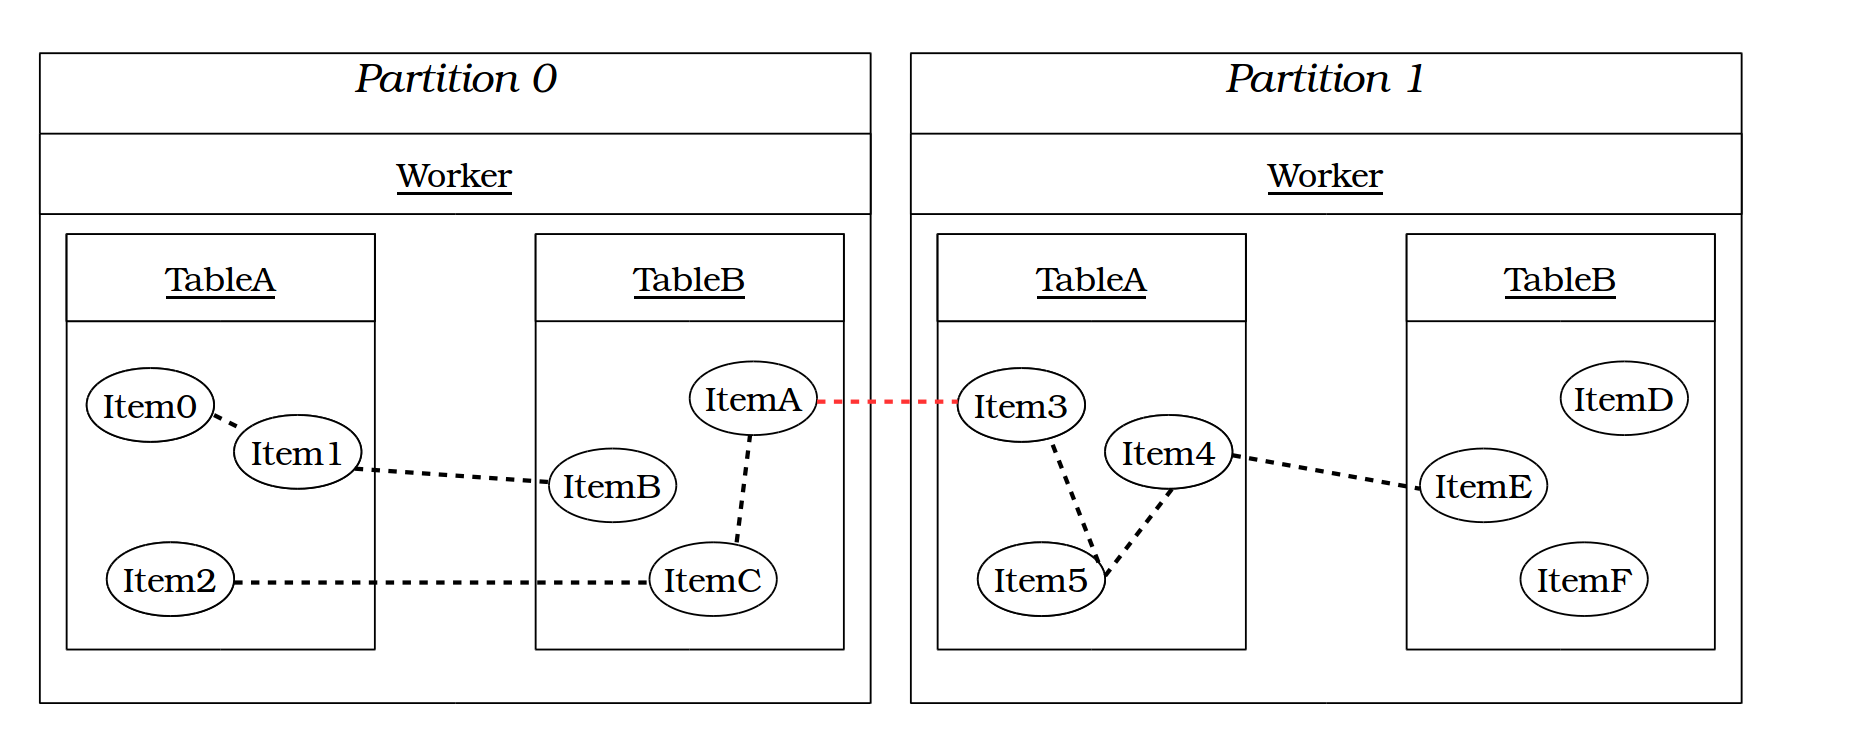
\includegraphics[width=15cm]{illustrations/png/basicmodel.png}
\caption{Overview of the organization of data structures in a Saddlebags application.}
\label{fig:basicmodel}
\end{figure}

The relation between items, tables and partitions are illustrated in figure \ref{fig:basicmodel}. This illustration shows a basic design of a Saddlebags application with two tables and two partitions. Underlined names are objects that exist on every partition. Lines indicate example communication, with red lines indicating communication between different partitions. Items of different types are stored in different tables, and the same tables are available on both partitions. Item names are unique across all partitions, and a single item have affinity to a single partition. 

Tables are stored within a \emph{worker}, a distributed object. Tables are referenced via this object. The behavior of the worker need not be extended by the programmer, and in the context of data flow and execution model the worker is relatively insignificant, and will be mostly ignored in this section. It will be explained further when discussing implementation and interoperability with UPC++.

Items implement a \emph{work-push-pull} model, in which \emph{work} refers to a computational task implemented in the item class, and \emph{push} and \emph{pull} are the two available modes of communication. The work of an item is designed to be executed iteratively, and each iteration of a Saddlebags application involves executing work and performing any communication routines that was called as a result of the work. An iteration applies to every item in every table, and it is with this iterative model that an application can be executed. 

\subsection{Events} \label{section:events}
The data flow model of Saddlebags is implemented with the concept of \emph{events}. Within the context of this framework, an event refers to the receiving of any communication message, or reaching specific points of the iteration process. Whenever an event is triggered, for example when receiving a \emph{pull} message, the item that received an event-trigger calls a corresponding method, in this case a \emph{foreign pull} method. The contents of this method can be implemented differently in different item types, and is also able to initiate other communication routines. This is directly related to the data flow of an application: when receiving a pull event, the event-triggered method determines what data to return. When the message returns to the original sender with some data, the event-triggered return method determines how to handle the data. 
\newpage

\begin{table}[h]
\setlength\arrayrulewidth{1pt}
\renewcommand{\arraystretch}{2}
\begin{tabular}{ | p{3cm} | p{6cm} | p{6cm} |}
   	\hline
   	\textbf{Method} & \textbf{Event} & \textbf{Implied data movement} \\ \hline
   	On Create & Item is created & None\\ \hline
  	Refresh & An item with the same name is attempted created & None \\ \hline
  	Work & Start of iteration & None \\ \hline
   	Foreign Push & A push message is received from another item & Data from sender is received with the message  \\ \hline
   	Foreign Pull & A pull message is received from another item & Return data is sent back to the sender\\ \hline
	Returning Pull & A pull message that originated in this item has returned & Data from pull target is received with the message\\ \hline
	Finishing Work & End of iteration & None\\ \hline

\end{tabular}
\caption{All events and their corresponding methods}
\label{table:events}
\end{table}
\vspace{1.5cm}

Table \ref{table:events} lists all methods in the item class that can be triggered by events. Column 1 lists the names of the methods, column 2 lists the circumstances under which the method is called, and column 3 lists what data is moved in the corresponding method.

All methods with data movement are called as a result of communication with other items. Communication routines can be initiated in any of the methods listed in the table. Items are referenced by name, so two items with the same name cannot exist in the same table. The \emph{Refresh} method is used to incorporate this behavior in a program.
\newpage
\subsection{Example: PageRank} \label{section:examplepagerank}
The programming model that is implied by items and events can be explained further through an example application. Consider the PageRank algorithm, a mathematical expression for ranking the importance of a website \cite{pagerank}. The following expression is a simplified way of calculating the Page Rank ($PR$) of a website ($u$), given a list of pages that link to it ($B_u$), and the total number of links from those websites ($N$):

\vspace{10pt}
\begin{center}
${\displaystyle PR(u)=\sum_{v\in B_{u}}{\frac{PR(v)}{N(v)}}}$

\end{center}
\vspace{20pt}

It is assumed that every page starts with a PageRank of 1. Given a list of pages and their outgoing links, a PageRank application can be designed with the Saddlebags programming model. Each page is implemented as an item, and each item is given a list of its own outgoing pages, in addition to a PageRank value and a buffer for calculating a new PageRank, set to 0. Only one table and one type of item is needed. The required methods are listed in table \ref{table:pagerankevents}. When the items are created, the algorithm can be ran for as many iterations of PageRank as needed, since one PageRank iteration (one execution of the aforelisted formula for each item) is equivalent to one Saddlebags iteration.

\vspace{1.5cm}

\begin{table}[h]
	\setlength\arrayrulewidth{1pt}
	\renewcommand{\arraystretch}{2}
	\begin{tabular}{ | p{3cm} | p{12cm} |}
		\hline
		\textbf{Method} & \textbf{Functionality} \\ \hline
		Work & Each page that this item links to will receive a push message with this item's PageRank divided by this item's count of outgoing links \\ \hline
		Foreign Push & Add the incoming value to the new PageRank buffer \\ \hline
		Finishing Work & PageRank of this item is set to the value of the buffer. The buffer is set to 0.\\ \hline
		
	\end{tabular}
	\caption{The methods required to implement PageRank with Saddlebags}
	\label{table:pagerankevents}
\end{table}

\section{Architecture and data flow}
\subsection{Table structure}
Programming a Saddlebags application involves two main tasks: extending item methods to fit a computational purpose, and creating items through data input. In the example illustrated in the previous section, table \ref{table:pagerankevents} shows the extension of an item, and feeding outgoing links to an item is an example of data input. Items are referred to by the name of the table that contains it, and the name of the item itself. This is the only way to reference an item in Saddlebags, as tables are responsible for both item initialization and storage.

A table represents an associative array, a collection of unique keys, and values, in which keys are item names and values are item object instances.  Tables are initialized with a name and an item type, and each table can only contain items of a single type. There can be an arbitrary number of tables in a program, and item types are not tied to a single table instance. It is guaranteed that one instance of all tables are available on all partitions.




\subsection{Data distribution}
Each table is initialized with a distributor type, a specific class with a distribution method that determines the partition in which items should be located. Since all data is stored in items, and all items are stored in tables, the distribution type of tables is the only component of a Saddlebags application that manages distribution of data and computation.

The distribution method that is common for all distributor classes takes an item name as parameter, and returns a partition identifier. By default, distribution is based on the hash digest of the item name, utilizing consistent hashing where items will be assumingly evenly spread around all partitions \cite{consistenthashing}. The motivation behind this is to distribute computational tasks as evenly as possible.

It is possible for different tables within the same program to use different distribution logic, since distributors are tied to tables. Figure \ref{fig:communication} shows an example application structure with two tables and two partitions. Table 1 in partition 0 sends a push message to an item in table 2, and the distributor in the instance of table 2 in partition 0 directs the message to partition 1. The initial message is only directed at a table and item, since this is the only information about the data layout that a programmer has access to. All tables are initialized on all partitions, so any table's distributor is available to all items. This enables communication between all tables and partitions.
\vspace{0.4cm}
\begin{figure}[H]
	\centering
	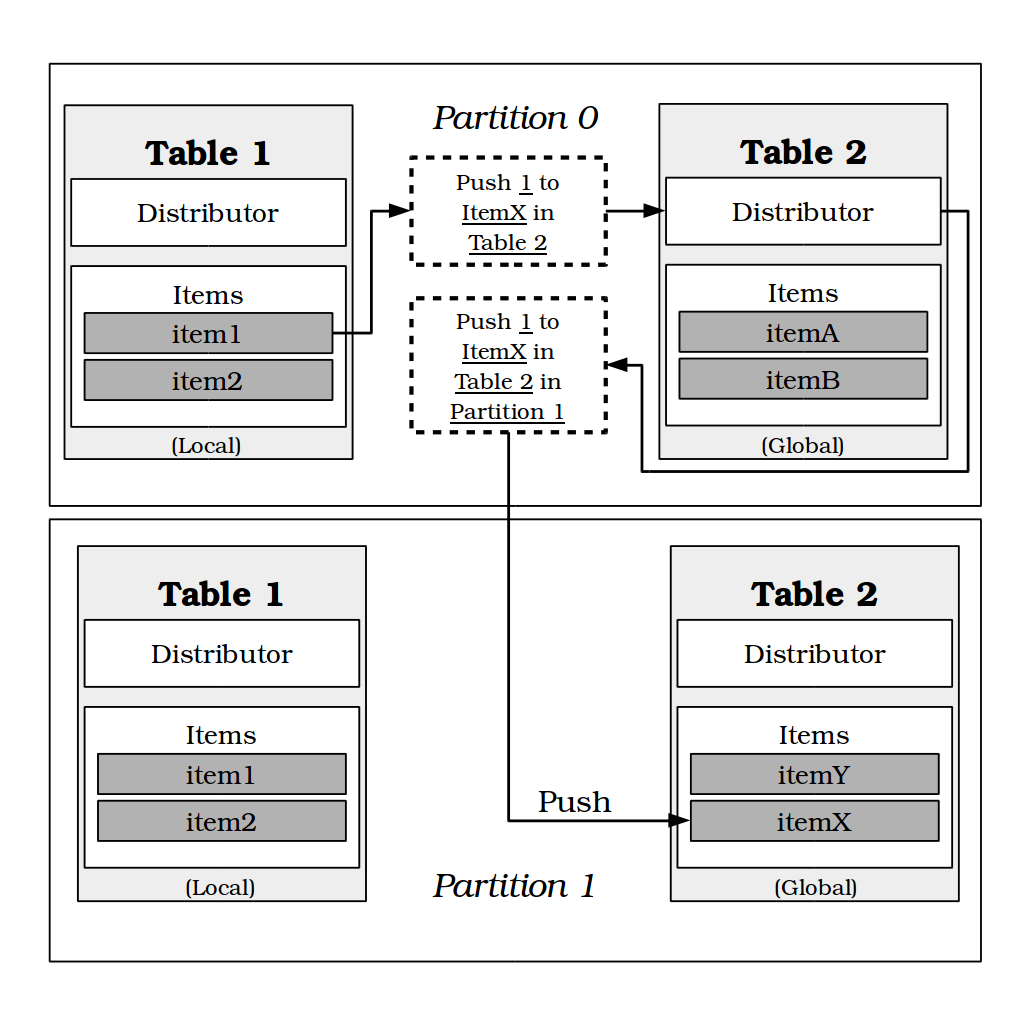
\includegraphics[width=13cm]{illustrations/png/communication.png}
	\caption{Example of communication between tables on different partitions.}
	\label{fig:communication}
\end{figure}

\subsection{Table locality}
When a table is created, it is specified whether it is a local or global table. Global tables utilize distributors, that can potentially distribute data across all partitions that are available in the system. Local tables does not utilize any distribution logic, and all items are stored within the same partition as they were created. While local tables are created on every partition, their items cannot be remotely accessed. The items in global tables can always be remotely accessed, regardless of their distribution~model.

Note that in figure \ref{fig:communication}, table 1 is classified as local, while table 2 is classified as global. Table 1 has the same item identifiers on both partitions, while table 2 has different items. If items with identical identifiers were added to table 2 from both partitions, they would still only be stored in one partition, as the distributor would redirect the item creation. If items with identical identifiers were added to table 1 from both partitions, each partition would get its own instance of an item with the same identifier. From a programming standpoint, communication with local or global tables looks identical, but setting the locality of a table can have an impact from a data movement and optimization standpoint, since communication with a local table will never implicitly invoke remote operations.


%The communication patterns of a push/pull paradigm is simple enough that the cost of data movement as a result of communication in an application can be reasoned about, despite implementation complexity being hidden. 

%Saddlebags is designed with the goal that abstractions provided by the programming model, through C++ mechanisms such as inheritance and type templates, should not affect algorithmic complexity. This will likely only be true for algorithms that can be tailored to the push/pull/work paradigm. 

\section{Fault tolerance}
Saddlebags takes an approach to achieving a degree of fault tolerance by utilizing replication. Each partition will act as a replica for one or more partitions with subsequent rank values, looping back to partition 0 at the highest rank. The degree of fault tolerance, i.e. the number of replicas per partition, is defined on a per-application basis. This is similar to the hash ring approach found in the key/value storage system Dynamo \cite{dynamo} and the peer-to-peer hash table protocol Chord \cite{chord}.

Replicas are updated at the end of each iteration, which means that every node is in a state where no updates occur when replication routines are executed. This makes for low communication overhead during replication, since all contents of a table can be sent in one message. This raises an issue with inconsistency, if a node crashes during computation. A situation like this must be solved with a rollback operation, moving every table to the previous iteration. This is achievable with the same replication routines, since a back-up of the state of the previous iteration exists in the current replicas. This means that, to rely on rollbacks, a replication degree of at least 2 must be used. 

Figure \ref{fig:ring} shows an overview of 8 nodes and their replicas, when a program is initiated with a fault tolerance degree of 2. Each letter A-H represents a node, partition, and part of the key space of the hash digests of item names.

\vspace{1.5cm}
\begin{figure}[H]
	\centering
	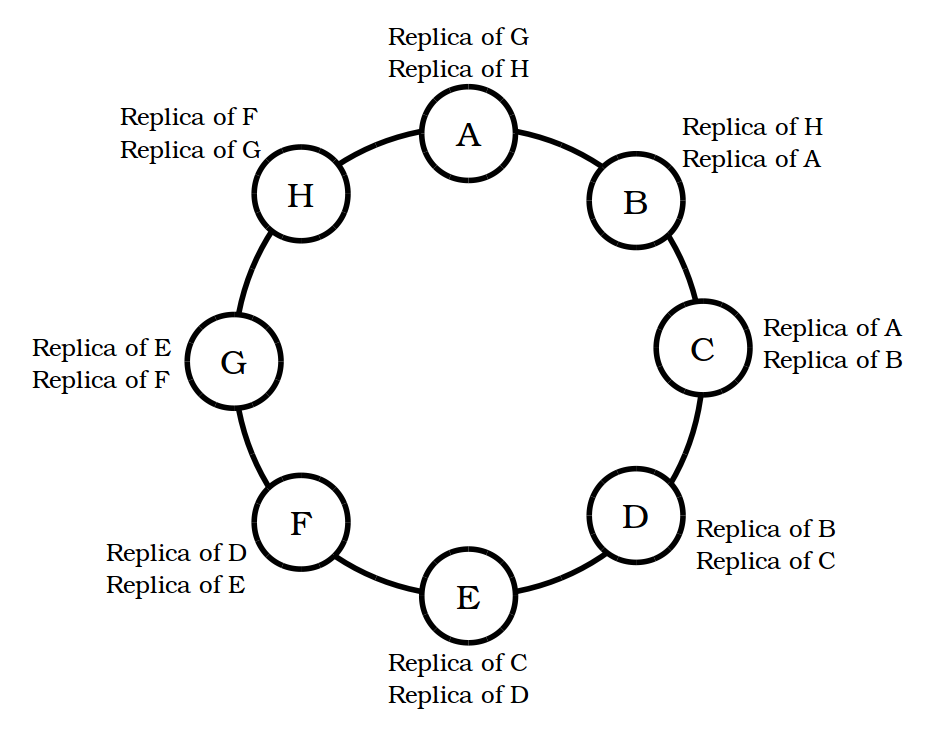
\includegraphics[width=12cm]{illustrations/png/ring.png}
	\caption{Hash ring-view of Saddlebags application with 8 nodes and a fault tolerance degree of 2}
	\label{fig:ring}
\end{figure}

\newpage
\mbox{}
\newpage
\chapter{Implementation}
This chapter will present the implementation of Saddlebags, explaining how the design translates into different data structures, and how programs can be written within this framework. Saddlebags was implemented in the C++ programming language, and it can be used to write parallel programs in C++ by importing its header file. Saddlebags is built on the UPC++ library for C++, and this library is a requirement in order to compile Saddlebags programs. Because of this dependency, Saddlebags poses the same system requirements as UPC++. In brief, it can be used on Linux with $gcc$, on macOS version 10.11 or newer, and on Cray XC supercomputers \cite{upcreq}. On Linux clusters with MPI support, UPC++ programs can be executed with MPI commands~\cite{upcmpi}.

\section{Overview}
The previous chapter presented an object-oriented approach to parallel computation, in which problems were split up into separate items that could be distributed and accessed independently of other items. Defining computational tasks in items, and passing data as messages between items with different tasks, is the main effort of implementing programs in Saddlebags. The final program structure of the framework was devised in the development of an interface in which items of different types were interoperable, through a common messaging interface.

Generic items are implemented as a C++ class, consisting of pre-defined communication methods, in addition to several empty methods, corresponding to the events listed in section \ref{section:events}. To develop meaningful programs, some of these events must be extended. This is done through inheritance. Event-methods are marked as \texttt{virtual}, so that they can be overridden. Non-event methods, such as push and pull, implement generic functionality that will remain the same for all item classes. This leaves the \texttt{virtual} methods to indicate the interface in which events can be implemented. 

Items are stored in hash maps, which are defined in a \texttt{TableContainer} class. The hash map and table container makes up the functionality of the table described in chapter~\ref{chapter:design}. \texttt{TableContainer} inherits from a \texttt{TableContainerBase} class that contains functionality that is applicable for all item types. The reason for this will be expanded on in section \ref{section:templates}. Table containers have default logic for distributing items across partitions, and this can be exchanged for specialized solutions by passing a \texttt{Distributor} object. The \texttt{Distributor} class implements a \texttt{Distribute()} method that takes a item key as parameter, and returns an integer corresponding to the rank in which that item should be stored. 

An application can consist of multiple tables, containing different item types. Tables are stored in the \texttt{Worker} class, which is responsible for synchronization, initiating computational tasks through the events \emph{Work} and \emph{Finishing work}, and providing a common interface for different items to access each other in order to deliver messages. Every table and item in a program can be referenced through its worker. A Saddlebags program is initiated by creating a worker, and there is little purpose in having multiple simultaneous workers.


%message class

The main classes in the Saddlebags implementation is shown as a UML diagram in figure \ref{fig:uml}. In practice, an application will have at least one additional class, inheriting from the \texttt{Item} class. 



\begin{figure}[H]
	\centering
	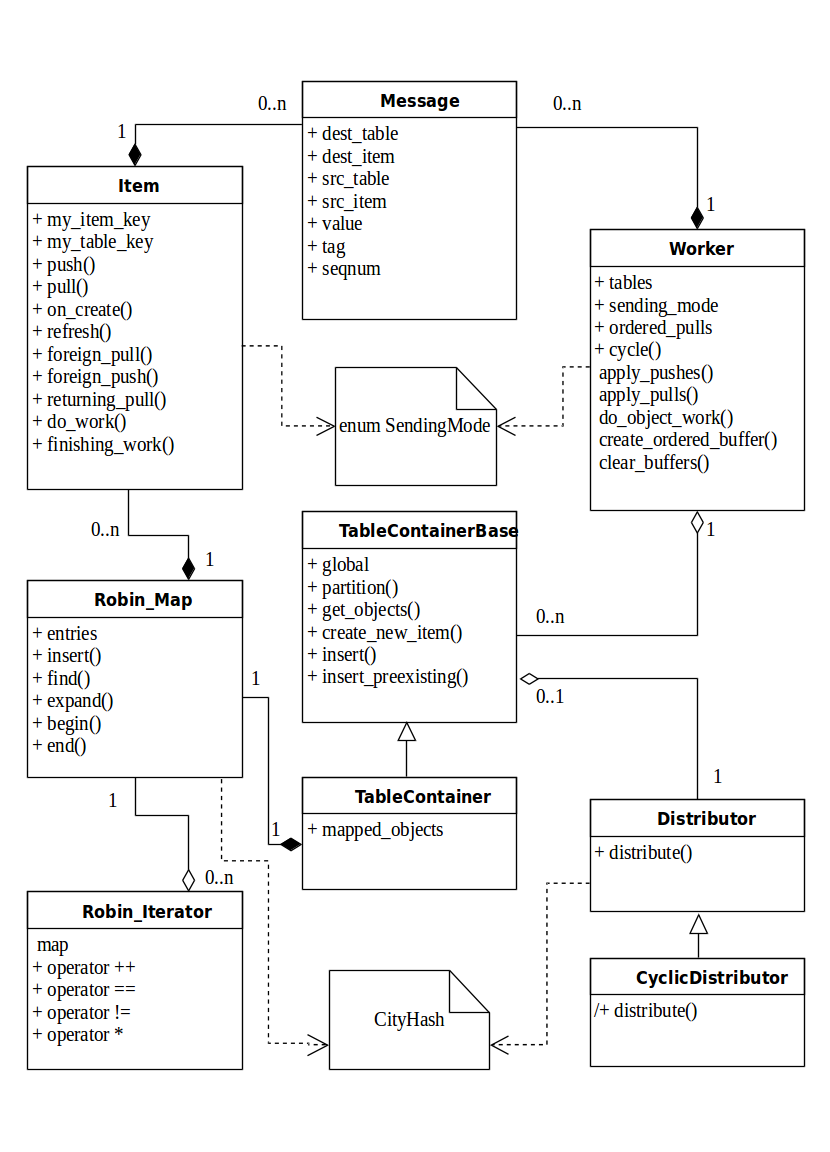
\includegraphics[width=15cm]{illustrations/png/uml.png}
	\caption{UML diagram of Saddlebags' main classes.}
	\label{fig:uml}
\end{figure}


\section{Template types} \label{section:templates}
Template programming is a feature of C++ that enables the use of generic types when defining classes and functions. A generic name can be used in place of a specific data type in the definition of a class or function, enabling more flexible declarations and reducing code duplication. When an object is initialized, generic types must provided, in addition to the regular constructor parameters. Template programming was used heavily in the implementation of UPC++ \cite{upc_language_specification}. Listing \ref{lst:template} shows an example of the syntax of declaring a template class with one template typed property, and declaration of a child class.

Template programming is used in the implementation of Saddlebags for two reasons. Firstly, to achieve a general-purpose programming model, a framework user should be able choose the data types that suits a particular problem. Secondly, the item extension model described in chapter \ref{chapter:design} requires the framework to be able handle different item classes.
\\ \\
\begin{lstlisting}[label={lst:template}, float=h,frame=tlrb, caption={Declaration and initialization of an inherited template class in C++}, captionpos=t, language=c++, showstringspaces=false]

template<class T>
class MyClass
{
  T value;
};

template<class T>
class MyChildClass : public MyClass<T>
{
  T otherValue;
};

auto obj = MyChildClass<int>();
obj.value = 34; //obj.value is of integer type
\end{lstlisting}
\newpage
\subsection{Parameters}

Every class listed in the diagram in figure \ref{fig:uml} is a template class. The \texttt{Worker}, \texttt{TableContainerBase}, \texttt{TableContainer}, \texttt{Item}, and \texttt{Message} classes take at least the three following template parameters.
\\

\hspace{4ex} \textbf{\texttt{TableKey\_T}}
\\
The type of the variables that tables are referenced by. Every table has a name that is stored with the same type, defined by this template parameter. The parameter is needed in the \texttt{Worker} class because references to all tables are stored here. It is needed by item classes because communication methods require a table name to reference other items to communicate with. It is needed in the \texttt{TableContainer} class because the table is responsible for initializing items. It is needed by the message class because the destination table and object must be stored in outgoing messages.
\\
 
\hspace{4ex} \textbf{\texttt{ItemKey\_T}}
\\
The type of the variables that items are referenced with in a table. A value of this type is used whenever an item is accessed. A worker and table can access items by looking up its key, and items can communicate with other items by initializing messages that contain item keys. Furthermore, items can only be initialized by passing an item key to the table.
\\

\hspace{4ex} \textbf{\texttt{Message\_T}}
\\
The type of the data that is communicated through messages, i.e. push and pull operations. The Message class itself has several fields, all of which are listed in the diagram in figure \ref{fig:uml}. However, the payload of this message is a single field of \texttt{Message\_T} type, which is delivered to push and pull methods. Messages are delivered to items between iterations, so other classes also require this template parameter because messages can be buffered on delivery. Optional methods for communicating data is explained in the next section, but this type determines the data type to send~regardless.
  
The \texttt{TableContainer} class takes an additional template parameter that is the item type stored in that table. Since multiple tables can have different item types, the item type is given only to the table. The item type of each table is transparent to the worker, so that it can store an arbitrary number of tables in its \emph{tables} hash map. This is achieved through referencing \texttt{TableContainer} instances as \texttt{TableContainerBase} types - a parent class that does not take an item type template parameter. This is possible because the only methods from an item that is relevant for a worker is the methods that are available in the parent item class. Tables are stored in a worker as values in an \texttt{unordered\_map} from the C++ standard library.

In practice, this means that the \texttt{Worker} class contains a map with the key type 
\texttt{TableKey\_T} and value type \texttt{TableContainerBase<TableKey\_T, ItemKey\_T, Message\_T>*}. This allows workers to store all tables, in actuality of different types derived from\\ \texttt{TableContainerBase}, within the same data structure. When a table is created, the pointer that is passed to a worker is of type \texttt{TableContainer<TableKey\_T, ItemKey\_T, Message\_T, ItemType<TableKey\_T, ItemKey\_T, Message\_T> >*}\\ replacing \texttt{ItemType} with a relevant child of the \texttt{Item} class.

Similarly, a table can be given a \texttt{DistributorType} as a template parameter to customize the distribution logic. This is also not present in the \texttt{TableContainerBase} class and is transparent to workers.

From this design, it seems possible to move the transparency of item types from the \texttt{Worker} to the \texttt{TableContainer}, relieving the need for the \texttt{TableContainerBase} class; the same logic that allows a worker to access tables from a common parent class also applies to accessing items from their parent class, since there is already need for at least one item child class. However, a parameter with the child item class is needed in the table because this is where items are initialized. The \texttt{TableContainer} class is responsible for initializing items because item keys are unique, and attempts to initialize an item with a pre-existing key will result in calls to the Refresh method rather than actual initialization, as shown in table \ref{table:events}.


% for two reasons: item types and generic framework
% templates in each class: tablekey itemkey messagetype
% table defined with inherited item class
% item class in table is transparent to worker, worker has basetablecontainer
% this allows aribtrary number of tables with any item class
% <listing of declaration of worker and table from pagerank (with strings as item key)>

% table could be used with base item type and no template since api is the same, but child item class is needed for initialization within table, and initialization in table is necessary since table ID is the only way to reference item

\section{Communication}
Partitions are executed in parallel, and the thread spawning and memory partitioning is handled by UPC++. Communication between partitions is achieved through UPC++ RPCs, in which a function is passed from one partition to another, where it is executed. As parameters, RPCs can use variables passed as value, or references to distributed objects from UPC++. In Saddlebags, partitions need to perform RPCs to initialize remote items, or perform remote pushes and pulls. For this, it is necessary for items to communicate with other items, even those in different tables. In order to achieve a design where every table can reference every other table, the worker is declared as the only distributed object in a Saddlebags program. The UPC++ Distributed Object class is a template class with a parameter to indicate the type of the target object. In this case, the distributed worker that can be used in RPCs is of type \texttt{upcxx::dist\_object<Worker<TableKey\_T, ItemKey\_T, Message\_T> >}. The underlying \texttt{Worker} object can be accessed using the dereferencing operator \texttt{*}.

A worker is initialized as a distributed object synchronously across all partitions, which is recommended by the UPC++ specification \cite{upc_language_specification}. Additionally, tables are created synchronously, to match the transparent distribution of items. With tables having a reference to the distributed worker, all items and tables can be referenced via RPC.

\subsection{Sending modes} \label{section:sendingmodes}
Communication between items based on push and pull methods. Saddlebags implements several different techniques for handling these communication routines, which is determined by a \texttt{sending\_mode} property in the worker. The following modes are implemented.
\newpage
\hspace{4ex} \textbf{\texttt{Buffering}}
\\
Push and pull operations are stored as messages, in which the table and item name of both the sender and receiver is stored. Messages are sent when the communication method is called, but received messages are buffered and not applied until after the work-phase is finished. The purpose of the buffering is to enforce a bulk synchronous parallel execution model.\\

\hspace{4ex} \textbf{\texttt{Combining}}
\\
Similar to the Buffering mode, but messages are not sent until the work-phase is completed, so that all messages with the same source and destination partitions are sent in a single RPC. This is implemented on the sender-side by buffering messages in an associative data structure with destination partition as key, and a vector of messages to that partition as value.\\

\hspace{4ex} \textbf{\texttt{Direct}}
\\
Operations are not stored intermediately as messages, but rather only expressed through the execution of its RPC. Does not enforce any synchronization, so push and pull operations can be executed both before or after work. \\

\hspace{4ex} \textbf{\texttt{GasnetBuffering}}
\\
Like the Direct mode, operations are only represented as an RPC. Like the Buffering mode, operations are performed in a bulk synchronous parallel pattern. This is achieved by not advancing UPC++ state, by not calling the \texttt{progress} function until all partitions has completed the work phase. This means that any buffering of operations is handled by the internal communication routines of GASNet. Other buffering techniques are preferred because GASNet cannot store more than 65536 outstanding operations \cite{gasnetpresentation}. This mode was implemented for the experimental purpose of removing the overhead of the Message abstraction.


\subsection{Ordering}
Messages are by default not received in a deterministic order. A configuration parameter can be set to execute returning pull-messages in the same order as they were sent out. Pushes does not have a defined desired order, since they, from the receiver's perspective, are sent in parallel from multiple items acting independently. Pulls has a defined desired order in which they are returned, and that order is the same that as they were sent out in. 

Ordered pulls functionality is implemented by each item creating a buffer for returning pulls equal to the size of outgoing pulls, and attaching a sequence number to every message before sending them. When a pull returns, the message is stored at the location in the buffer equal to its sequence number. This results in an ordered list of pulls. This approach is possible because the total number of outgoing messages is known at a point before any messages return, so that the buffer can be created with the desired size ahead of time.

It is not possible to order pulls using the \texttt{Direct} sending mode, because in this mode, some messages can be returned before all messages have been sent. It is also not possible to order pulls with the \texttt{GasnetBuffering} sending mode, since the ordering techniques require using the message data structure. 

%rpc, distributed object
%caching futures
%message
%sending modes!

\section{Table}
Items are stored in a hash table, which is implemented with a Robin Hood Hashing model~\cite{robinhash}. This hash table design is based around open addressing, meaning that all entries are stored in a single contiguous array, and linear probing, meaning that hash table collisions during insertions are handled by attempting to perform the insertion in the next entry in the array instead. When performing linear probing, a Robin Hood table will swap entries if the item that is currently being inserted is further from its desired position than the item in the entry that the probe is inspecting.
\newpage
For the correctness of the program, the necessary factors are the hash maps semantics: one-to-one association between keys and item instances, and the functionality of iterating through the map, accessing each item once. Further implementation details about the hash table are optimization decisions. Robin Hood hashing was chosen because it demonstrates a lower worst-case lookup time in comparison to other common designs, including the unordered map from the C++ standard library  \cite{hashbenchmark}. A custom hash table implementation was used so that parameters such as maximum load factor and initial table size could be tweaked for optimization.

The item type of a specific table is transparent to its worker, which is the object that a programmer will primarily interact with. A function is provided that returns a C++ iterator to the hash table in which entries, which are pointers to a child of the \texttt{Item} class, are reinterpreted to the actual child item type. This allows a programmer to use C++ iterators to lookup all items stored in a partition, without only using references to objects of the parent item type, which is what is provided to workers.

\section{Synchronization}
The only synchronization mechanisms adopted in Saddlebags are barriers and futures. UPC++ programs consist of a fixed number of threads, in which only one thread has access to each private memory segment. Multiple threads per UPC++ partition can be achieved with libraries such as OpenMP \cite{openmp}, but this technique is not used in Saddlebags. This means that sequential data structures can be used internally in the framework, since each partition contain their own instances of objects. For example, the hash table implementation does not contain any synchronization mechanisms or other parallel features. Pitfalls like hash table expansions during insertions, or insertions to the same hash table entry, are resolved by only calling UPC++ Progress in-between atomic operations. It is guaranteed that entire RPCs will be completed before yielding control back to the main execution of a partition. Calling progress to resolve outstanding operations is handled internally and is not the responsibility of a Saddlebags user.


% no synch for expansion etc due to progress
% one way communication futures are stored
% barriers in cycle
%
%\section{Usage}

\newpage
\chapter{Evaluation}
This chapter will provide an overview of the features and performance of Saddlebags in comparison with other systems. Section \ref{section:programmability} focuses on programmability features, providing an overview of the features that are available when expressing algorithms in bulk synchronous parallel frameworks, comparing Saddlebags, Husky and Pregel.

Section \ref{section:performance} will provide experimental performance comparisons with other systems, through PageRank and Term Frequency-Inverse Document Frequency benchmarks in Saddlebags, Spark and Husky.

Section \ref{section:configuration} provides experimental performance comparisons between different configurations of a Saddlebags application, providing an overview of the expected performance penalties of sending modes and message ordering.

\newpage
\section{Programmability}\label{section:programmability}
This section will overview of the programmability of Saddlebags in comparison with other systems with similar data distribution and execution models, namely Pregel and Husky. Both of these frameworks provide examples of implementations of the PageRank algorithm in their papers \cite{husky, pregel} to demonstrate programming models, and therefore this application is used as a baseline for a comparison of programmability. The PageRank algorithm was explained more in-detail in section \ref{section:examplepagerank}. Listing \ref{lst:pagerankhusky} contains C++ code for definition of a PageRank vertex in Husky, taken from an official repository of Husky example programs \cite{huskyexample}. Listing \ref{lst:pageranksaddle} contains C++ code for a PageRank item class in Saddlebags. Listing \ref{lst:pagerankpregel} contains C++ code for a PageRank vertex class in Pregel, taken from the Pregel paper. 

\begin{lstlisting}[label={lst:pagerankhusky}, float=h!,frame=tlrb,numbers=left, caption={PageRank vertex class in Husky}, captionpos=t, language=c++, showstringspaces=false]

class Vertex {
  public:
  using KeyT = int;
  Vertex() : pr(0.15) {}
  explicit Vertex(const KeyT& id) : vertexId(id), pr(0.15) {}
  const KeyT& id() const {
    return vertexId;
  }
  friend husky::BinStream& operator<<(
         husky::BinStream& stream,const Vertex& u) {
    stream << u.vertexId << u.adj << u.pr;
    return stream;
  }
  friend husky::BinStream& operator>>(
         husky::BinStream& stream, Vertex& u) {
    stream >> u.vertexId >> u.adj >> u.pr;
    return stream;
  }
  int vertexId;
  std::vector<int> adj;
  float pr;
};
\end{lstlisting}

\begin{lstlisting}[label={lst:pageranksaddle}, float=h!,frame=tlrb,numbers=left, caption={PageRank item class in Saddlebags}, captionpos=t, language=c++, showstringspaces=false]

class SiteItem : public saddlebags::Item<int, int, float> {
  public:
  float page_rank = 1;
  float new_page_rank = 0;
  std::vector<int> links;
  void do_work() override {
    for(auto it : this->links) {
      this->push(0, it, page_rank/((float)links.size()));
    }
  }
  void foreign_push(float val) override {
    new_page_rank += val;
  }
  void finishing_work() override {
    page_rank = new_page_rank;
    new_page_rank = 0;
  }
};
\end{lstlisting}

\begin{lstlisting}[label={lst:pagerankpregel}, float=h!,frame=tlrb, numbers=left,caption={PageRank vertex class in Pregel}, captionpos=t, language=c++, showstringspaces=false]

class PageRankVertex : public Vertex<double, void, double> {
  public:
  virtual void Compute(MessageIterator* msgs) {
    if (superstep() >= 1) {
      double sum = 0;
      for (; !msgs->Done(); msgs->Next())
        sum += msgs->Value();
      *MutableValue() = sum;
    }
    if (superstep() < 30) {
      const int64 n = GetOutEdgeIterator().size();
      SendMessageToAllNeighbors(GetValue() / n);
    } else {
      VoteToHalt();
    }
  }
};

\end{lstlisting}
\newpage
In terms of code length, all three frameworks are similar. Husky shows the longest class definition, at 23 lines of code, and Pregel shows the shortest, with 18 lines of code. This can likely be considered insignificant. A large portion of the Husky class is used to define communication routines with stream objects. Saddlebags and Pregel avoids having to explicitly define specialized communication routines, by using a template parameter to define a specific messaging type. In this example, Saddlebags uses floats, while Pregel uses doubles.

Both Saddlebags and Pregel define the computational task within the class. The Pregel class defines a single method, \texttt{Compute}, that contains all application-specific logic. Saddlebags splits this into several methods: work before communication, methods to call as a result of communication, and work after communication. Pregel's \texttt{Compute} allows iteration over all incoming messages, a feature that in Saddlebags is available through the \texttt{foreign\_push} and \texttt{foreign\_pull} methods. These methods are equivalent to message iterator code blocks in Pregel.

Messages that are delivered in the \texttt{Compute} method in Pregel is equivalent to push-messages in Saddlebags, and it is in both frameworks implemented in the receiver how to handle these messages. Saddlebags' pull messages and \texttt{foreign\_pull} method does not have an equivalent implementation in Pregel. Instead, each vertex has a defined \texttt{MutableValue} that can be fetched by other vertices, and it is assumed that a vertex will always transfer the same data item. In Saddlebags, what value is fetched is defined by the receiver. The Saddlebags approach offers more flexibility, at the cost of implementation complexity. In Saddlebags, all data properties in an item must be defined per-application, and there are no implicit assumptions about what data to return on incoming pulls, save for the template parameter \texttt{Message\_T}. Both Saddlebags and Husky explicitly defines a variable \texttt{pr} or \texttt{page\_rank} for storing relevant data, while in Pregel, only the \texttt{MutableValue} property is used.

The number of iterations of the algorithm to perform is expressed in the Pregel class through the \texttt{supersteps} function. Neither Saddlebags nor Husky has this expressed, and must rely on other parts of the program to initiate iterations and manage termination. A larger portion of the runtime of the algorithm is expressed in Pregel vertices than in Husky vertices and Saddlebags items, as it is able to define data, computational task, and termination, with some implicit communication routines. Saddlebags items are able to define data, computational tasks, and communication routines. Husky vertices can express data, and communication routines. Notice that in this example, the mathematical PageRank algorithm and initiation of messaging is not implemented in the Husky class, and is deferred to the main function of the program, after vertices has been created. However, this differentiation of computation code is only semantic, as all three frameworks distributes execution of tasks to the same computing units as where the relevant data items are stored.

Expressiveness features are difficult to quantify, and is in this comparison presented through observation of code examples and design overviews. The findings are shown in table \ref{table:programmability}. "Per application" refers to features that can be expressed, but are not present by default.


\begin{table}[b!]
	\begin{center}

	\setlength\arrayrulewidth{1pt}
	\renewcommand{\arraystretch}{2}
	\begin{tabular}{ | p{4cm} | p{3.5cm} | p{3.5cm} | p{3.5cm} |}
		\hline
		\textbf{Functionality} & \textbf{Saddlebags} & \textbf{Pregel} & \textbf{Husky}\\ \hline
		\textbf{Implicit distribution of data} & Yes & Yes & Yes \\ \hline
		\textbf{Message types} & push/pull & push/pull & push/pull \\ \hline
		\textbf{Payload of messages} &Return values of methods  & One common data element & Per-application definition of in/out streams\\ \hline
		\textbf{Ordering of messages} & Available, for pulls & No & No \\ \hline
		\textbf{Computation code} & In item, in multiple stages, in methods & In vertex, in one stage, in method & Defined in main program, iterating over vertices \\ \hline
		\textbf{Terminate on convergence} & No & Yes (explicit in task) & No \\ \hline
		\textbf{Adjacent vertices} & Per-application & Yes & Per-application \\ \hline
	\end{tabular}
	\caption{Features of item/vertex objects in Saddlebags, Pregel and Husky}
	\label{table:programmability}

	\end{center}
\end{table}

\section{Performance evaluation} \label{section:performance}
Benchmarks were performed on three different systems:

The first system, a desktop machine, has an Intel Core i5-4460 CPU @ 3.20 GHz, with 4 cores and 256 KiB, 1 MiB and 6 MiB L1, L2, and L3 caches respectively. This system has 8 GB memory and runs Ubuntu 16.04.

The second system, a university provided server, has an Intel Xeon E5-2650L v3 CPU @ 1.80GHz, with 24 cores and 768 KiB, 3 MiB and 30MiB L1, L2, and L3 caches respectively. This system has 64 GiB memory and runs CentOS 7.5.1804.

The third system is the Abel computing cluster at the University of Oslo. Abel consists of 650+ compute nodes, with Intel E5-2670 CPUs @ 2.6 GHz, with 16 cores and 64 GiB memory. At this time, Abel uses CentOS 6 \cite{abel}. Nodes are connected with FDR InfiniBand. In this evaluation, only one core is used per node. This is the default behavior of the workload manager available on this cluster \cite{abeluserguide}, and the recommended way of running Spark jobs \cite{abelspark}. 

This selection of systems is used because it allows for both single node and distributed workloads. The 4-core Ubuntu system is used because of compatibility issues with Husky and its dependencies and CentOS. The 24-core server is used so that single node benchmarks can be ran with more than 4 partitions.

PageRank and TF-IDF are used as benchmarks. This selection is discussed further in chapter \ref{section:discussion}. PageRank benchmarks were performed on Kronecker graphs. Kronecker graphs are graphs modeled after properties from real networks, with the purpose of providing a scalable generative mathematical graph model \cite{leskovec2010kronecker}. For this evaluation, Kronecker graph generation was performed with the BigDataBench benchmark suite \cite{wang2014bigdatabench}. This Kronecker graph generator accepts an input of the number of iterations to perform the generation algorithm. Graphs nodes are represented as 32 bit integers. The iteration count, in addition to the total size of the graph, is given in each individual benchmark result.

\newpage
\subsection{Husky} \label{section:huskycomp}
A comparison with Husky was ran on the desktop system. A PageRank example program, parts of which were shown in section \ref{section:programmability}, from the official Husky repository was used. Husky was launched with 4 workers, which is equivalent to 4 parallel threads. Saddlebags was launched with 4 partitions, and uses the default sending mode, which is \texttt{Buffering}.

Results are shown in figure \ref{fig:huskypagerank}. In this benchmark, Saddlebags completed the task in shorter time than Husky on three different Kronecker graphs. It is shown that both the base execution time, and the scaling with dataset size, are slower in Husky than in Saddlebags.

\vskip 2cm

\begin{figure}[H]
	\centering
	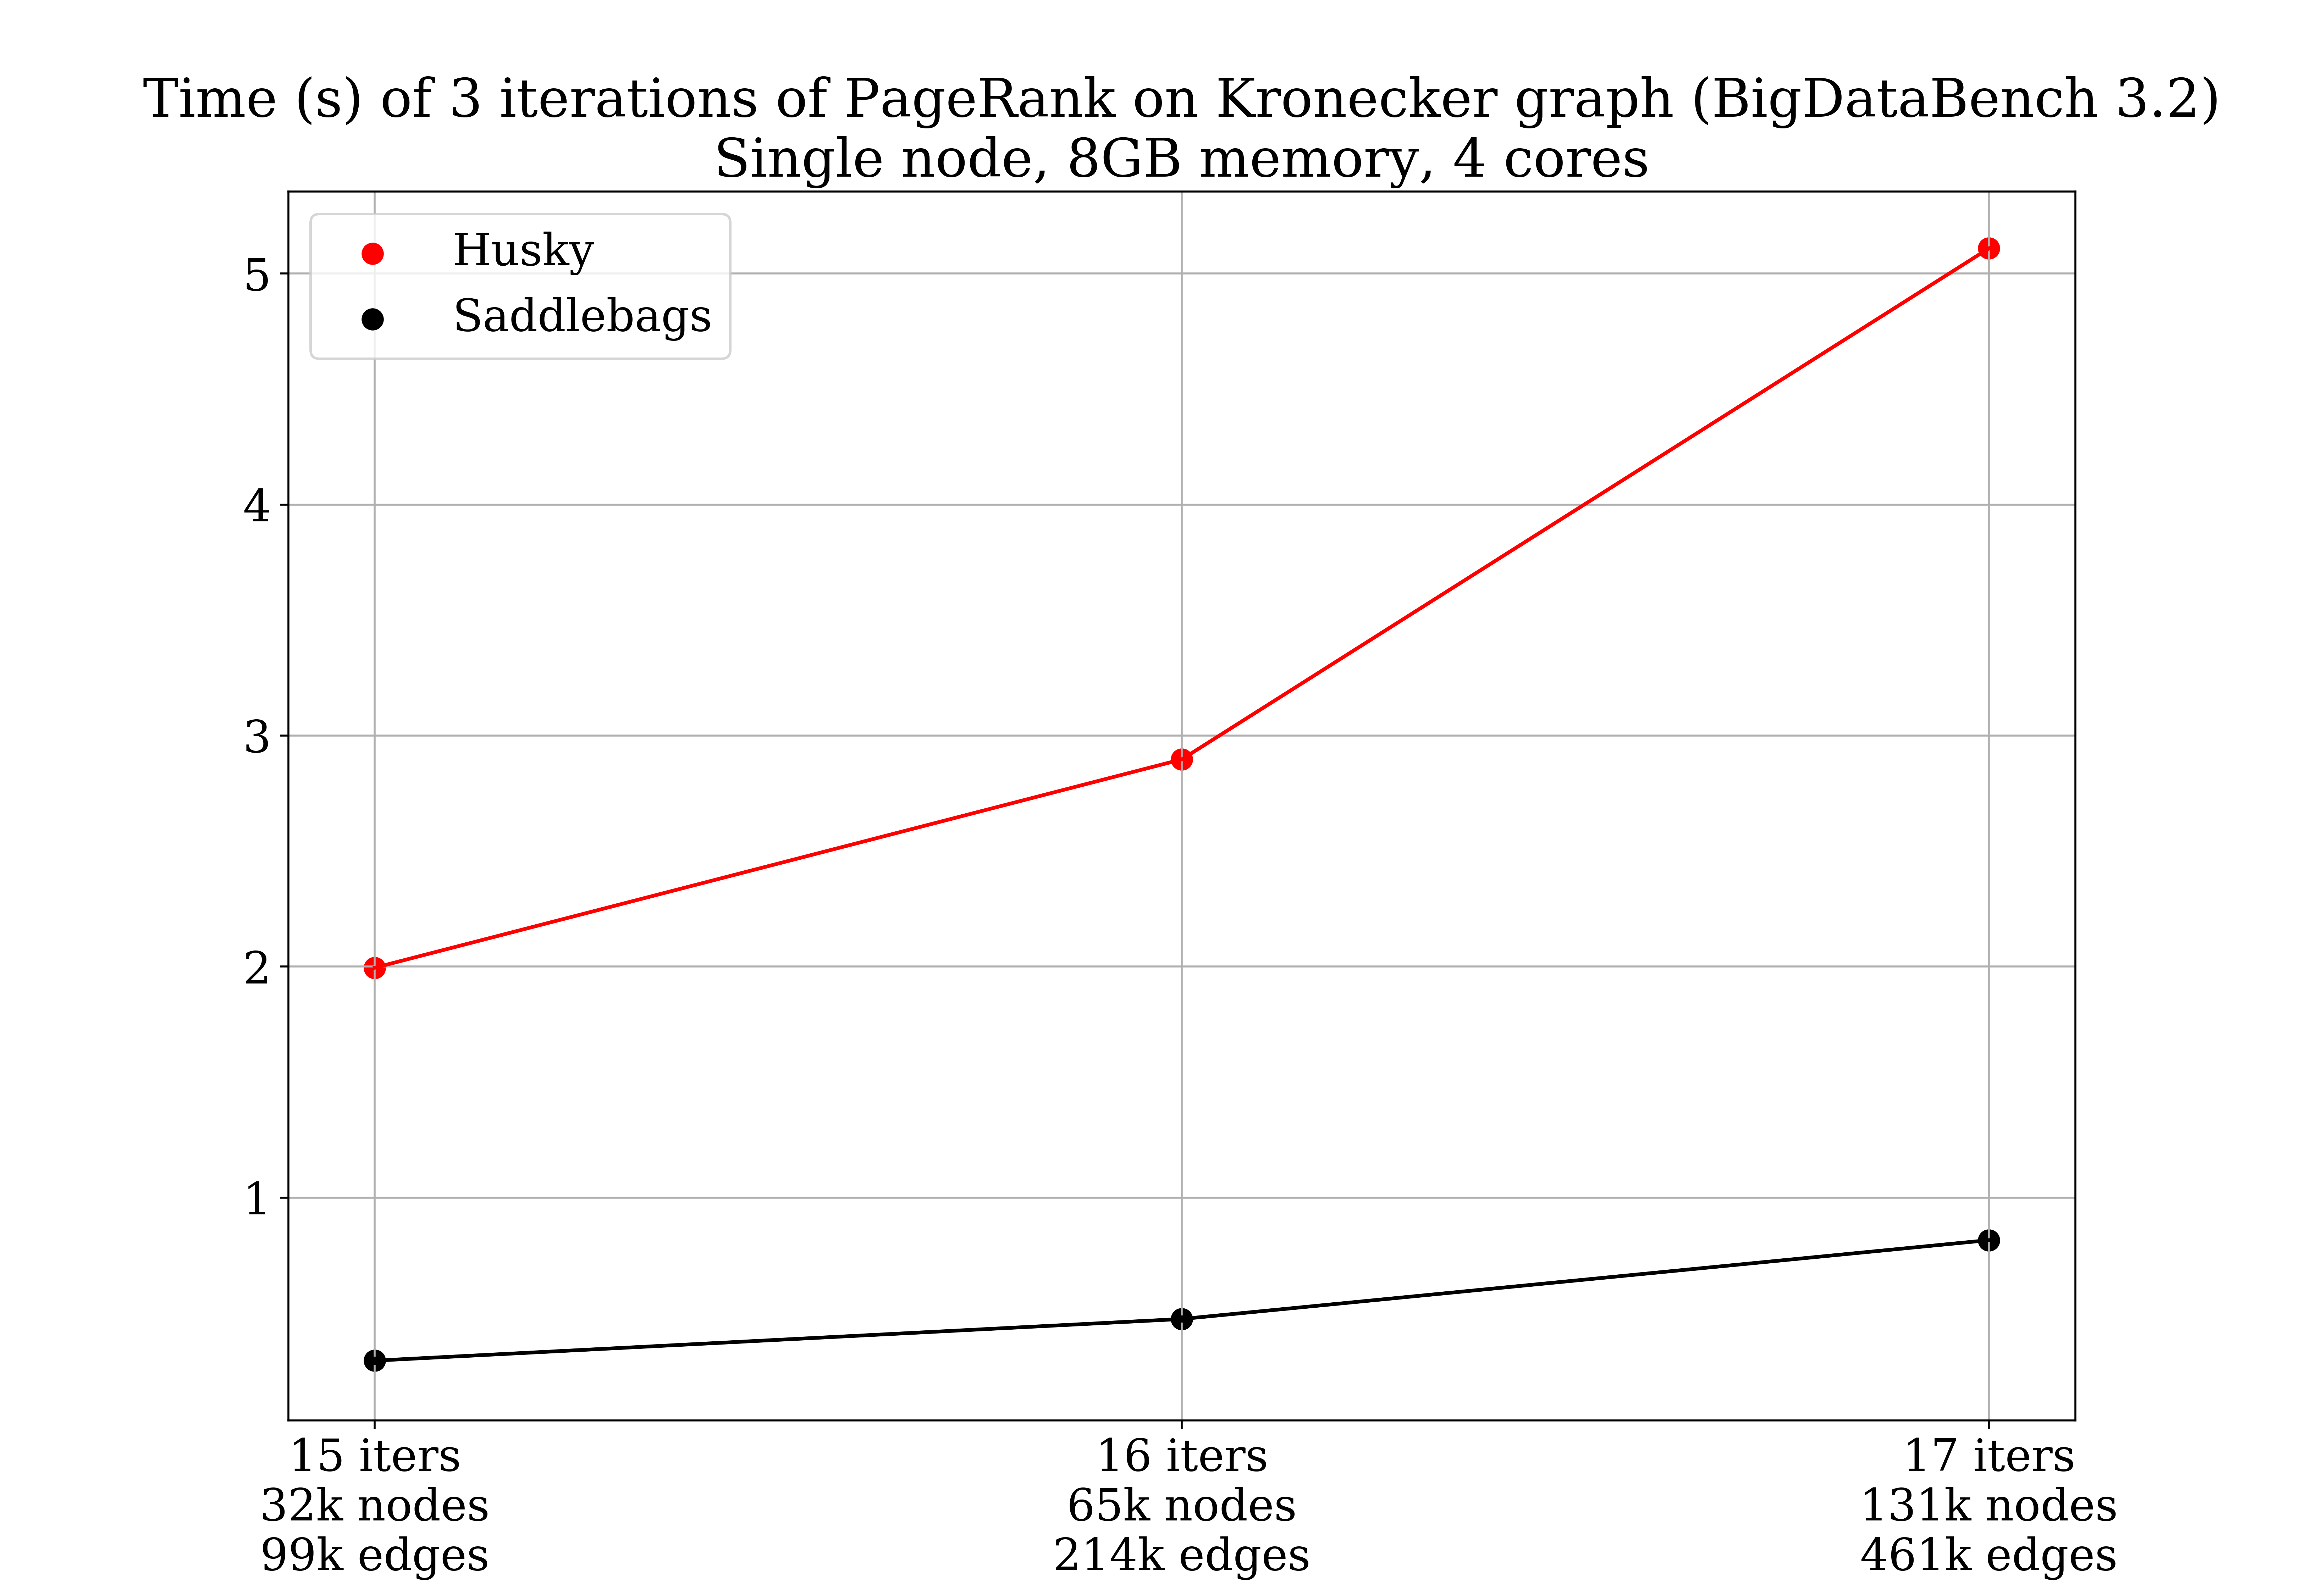
\includegraphics[width=15cm]{illustrations/png/huskypagerank.png}
	\caption{Execution time of PageRank in Saddlebags and Husky}
	\label{fig:huskypagerank}
\end{figure}



\newpage
\subsection{Spark}\label{section:sparkeval}
Comparisons with Spark were ran on the Abel cluster. For the PageRank benchmark, both a native Spark RDD MapReduce implementation, and a GraphX implementation, was used. GraphX is an API for running graph-based parallel jobs in Spark \cite{graphx}. Both the MapReduce \cite{sparkpagerank} and GraphX \cite{graphxpagerank} implementations were provided by official repositories. In thethe Spark implementation it is recommended to utilize GraphX to process this particular workload.

The other benchmark used with Spark is Term Frequency-Inverse Document Frequency (TF-IDF) \cite{tfidf}. This is an algorithm for classifying the relevance of words within a set of documents. A given word's importance within a given document is ranked based on its frequency within that document, and the inverse of the frequency of which it occurs in other documents. This benchmark was performed on a corpus of Wikipedia articles.

Results are shown in figures \ref{fig:pagerankspark} and \ref{fig:tfidfspark}. Both experiments show results that are significantly in favor of Saddlebags. These results are consistent with those presented in the Husky paper \cite{husky}, when using the comparison between Saddlebags and Husky from section \ref{section:huskycomp} as baseline. The advantage over Spark is explained by Husky as the result of fine-grained access of mutable data, which is also a relevant factor for Saddlebags, and applies to both benchmarks.

It can be inefficient to express communication through a network graph with only coarse grained parallel operations, as nodes can communicate with remote nodes regardless of the distribution of data. Similar issues arises with the TF-IDF algorithm, in which a distribution of documents across compute nodes is intuitive. Since the total occurrences of words across all documents is a relevant data item when calculating the final TF-IDF value, communication across compute nodes is unavoidable with this algorithm. The difficulty with these algorithms illustrates the merits of fine grained remote data access.

\newpage
\begin{figure}[H]
	\centering
	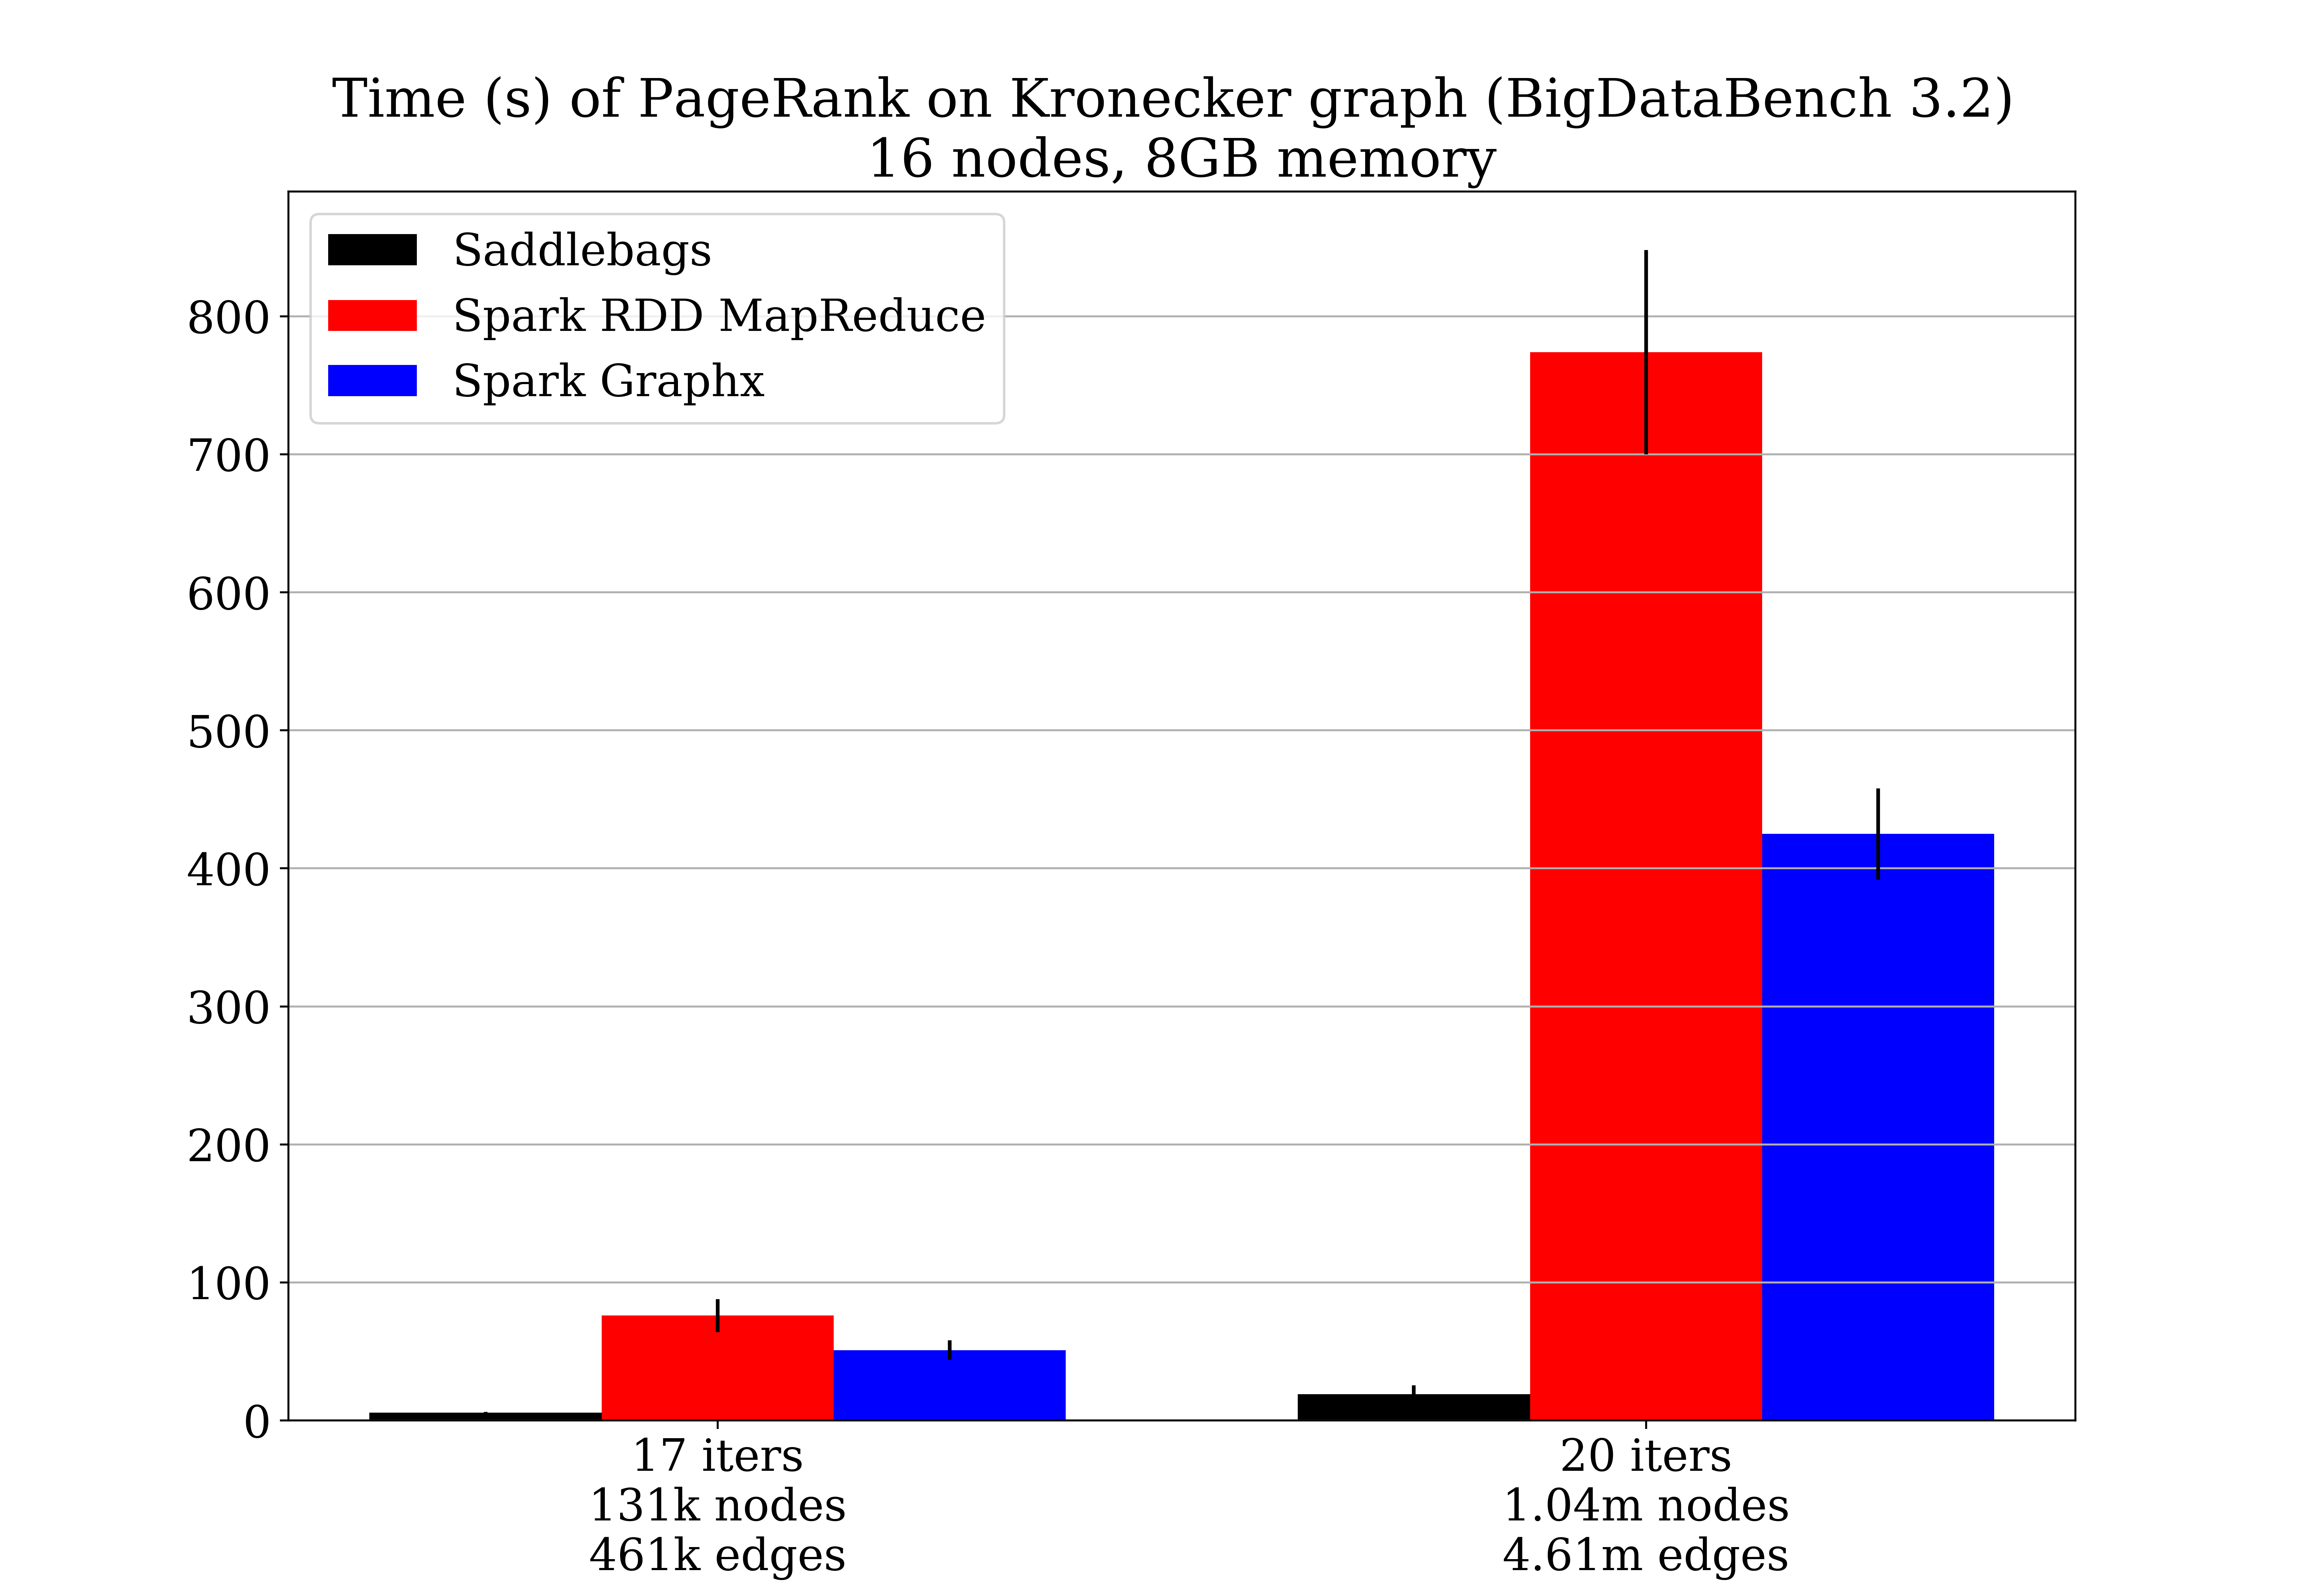
\includegraphics[width=15cm]{illustrations/png/sparkpagerank.png}
	\caption{Execution time of PageRank in Saddlebags and Spark}
	\label{fig:pagerankspark}
\end{figure}

\begin{figure}[H]
	\centering
	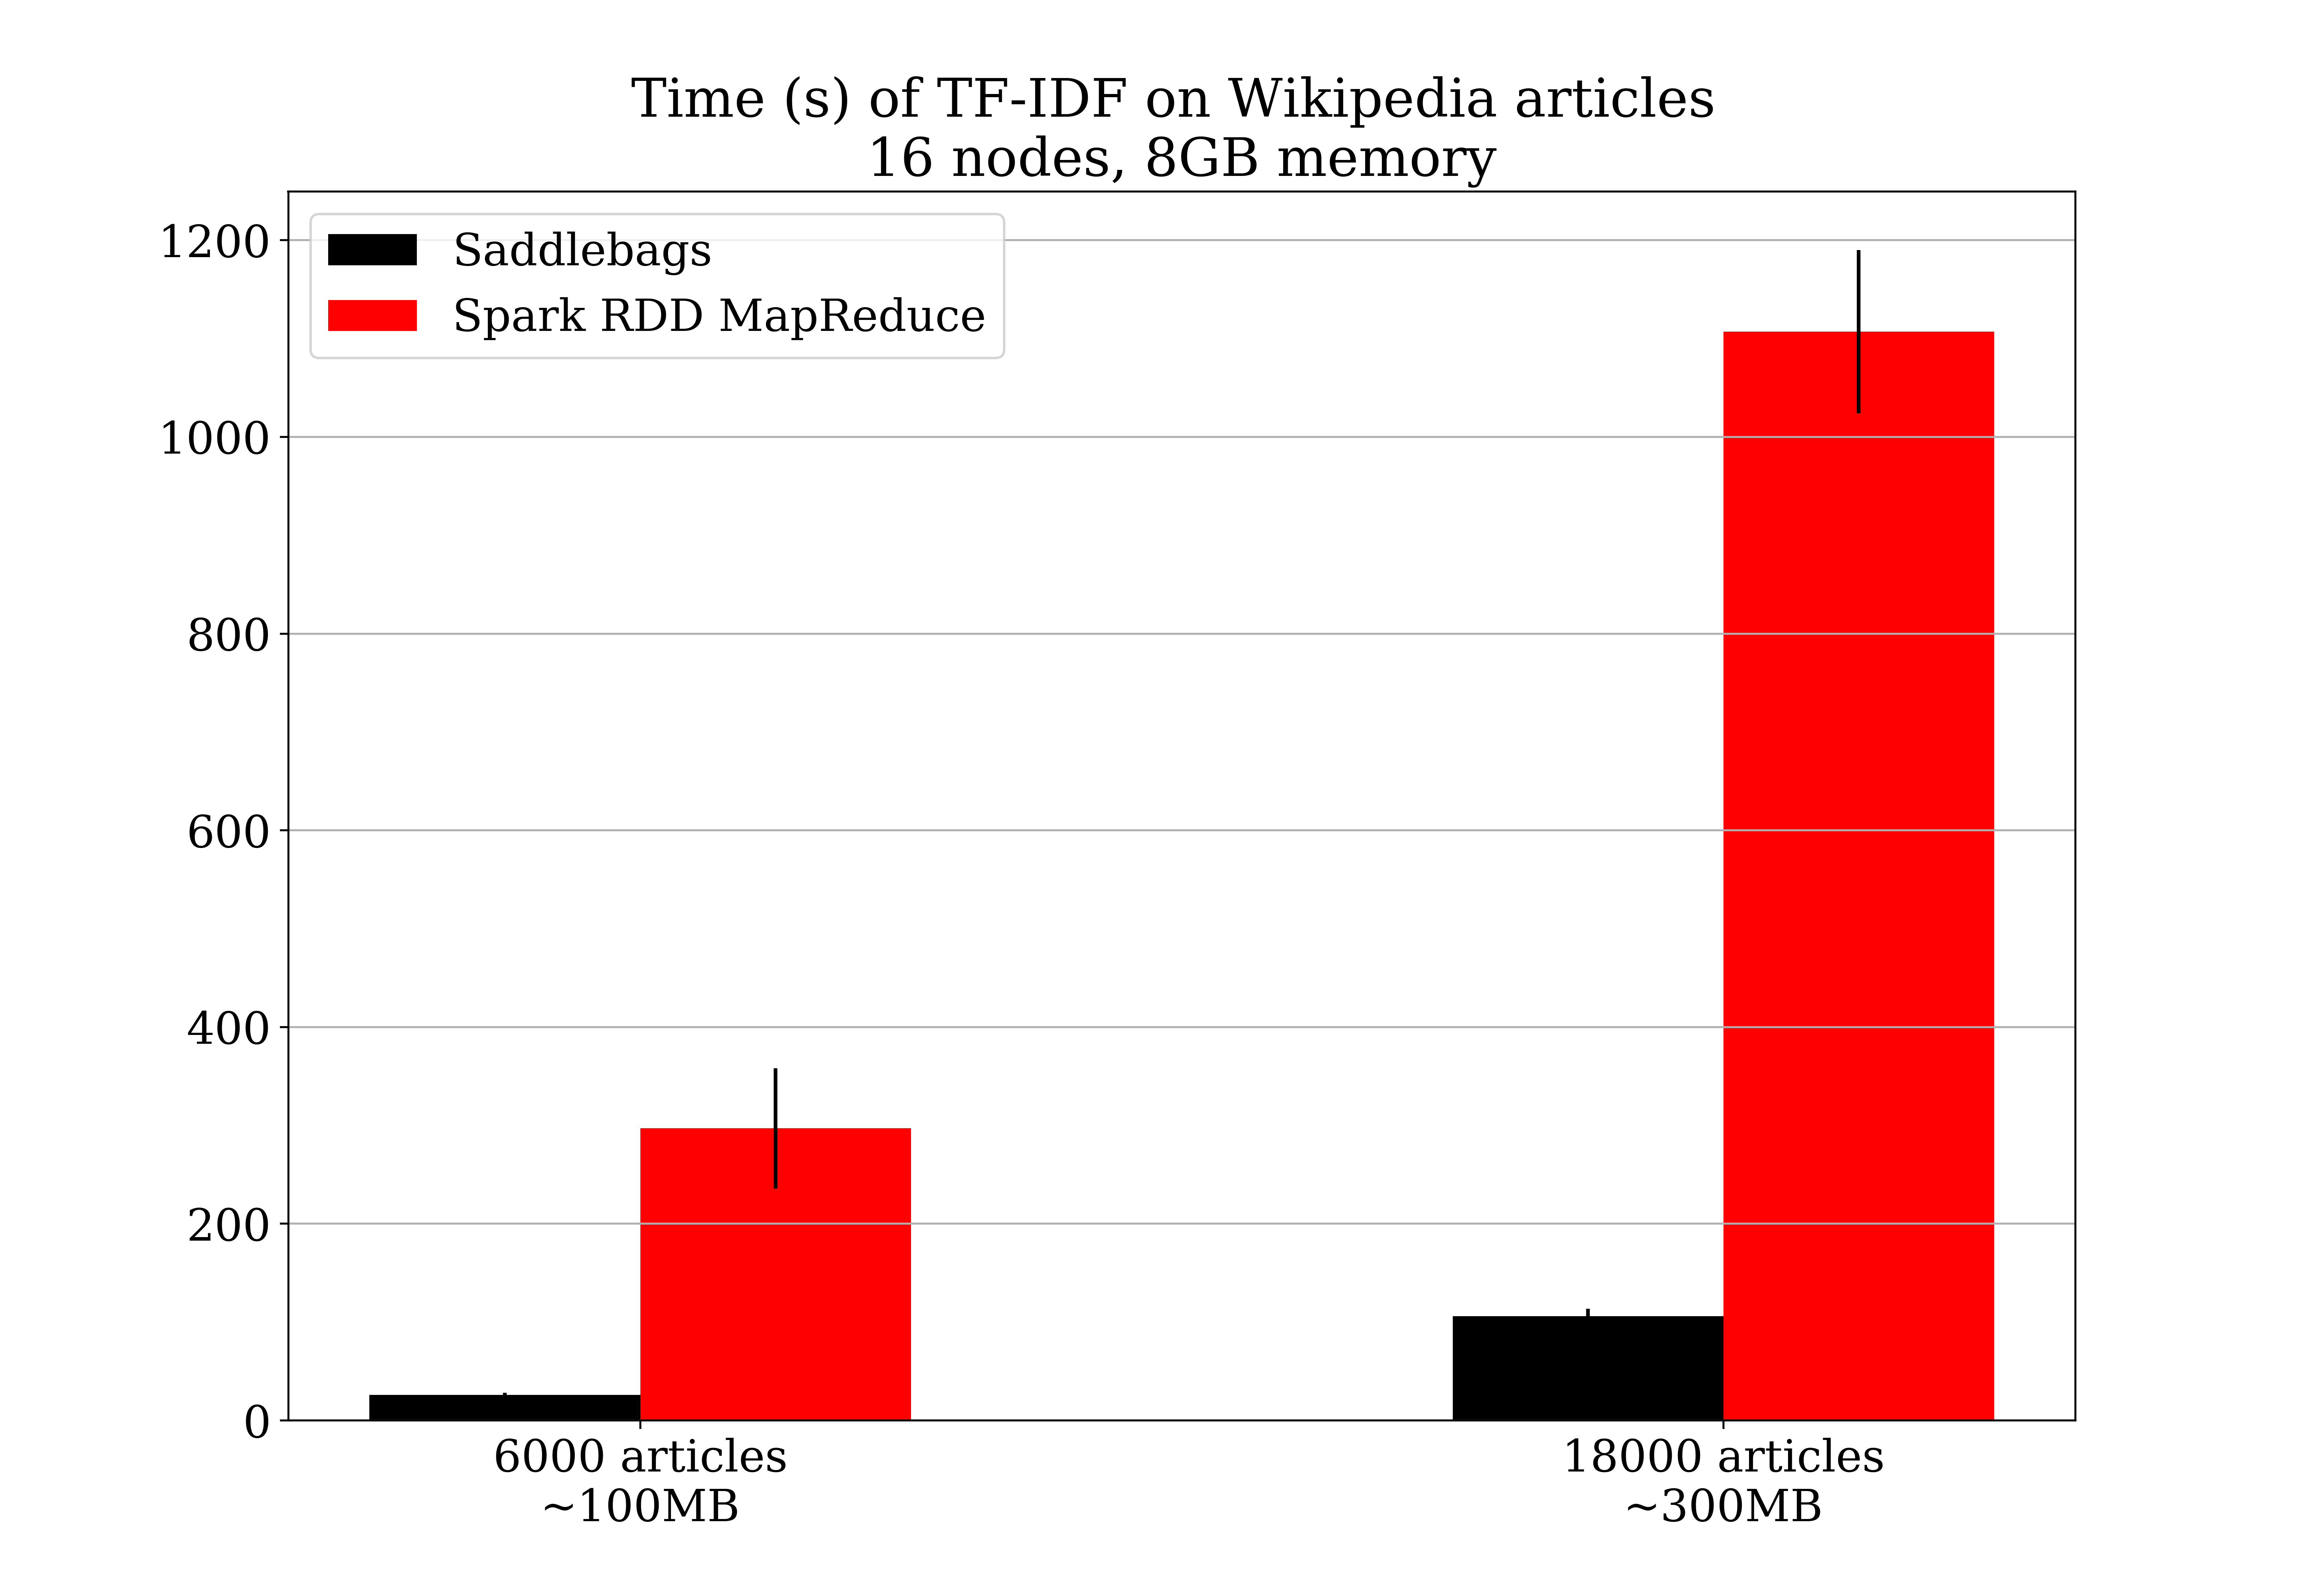
\includegraphics[width=15cm]{illustrations/png/sparktfidf.png}
	\caption{Execution time of TF-IDF in Saddlebags and Spark}
	\label{fig:tfidfspark}
\end{figure}
\newpage
\subsection{Fault tolerance}\label{section:replicationeval}
The PageRank experiment from section \ref{section:huskycomp} was performed again with replication enabled, and the results are shown in figure \ref{fig:huskyfaulttolerance}.
The increase in execution time of the algorithm per degree of replication can be analyzed with linear regression. The relationship between average execution time and degree of replication on 17 iterations of the Kronecker graph can be mapped to the linear equation $Y = 0.1945X + 0.8445$ where $X$ is degree of replication and $Y$ is total execution time, with $r^2 = 0.984$, suggesting that this model is a good fit for the data. In practice, this means that adding a degree of replication in this experiment will increase the execution time with 0.1945 seconds, which is 23\% of the base execution time. While the time measurements are specific to this experiment, the significant observation is the linearity of the increase in time per replica. The implementation of the replication routine also implies that the increase in time should be linear, because the additional data movement required per additional replication node is constant.
\vskip 0.5cm
\begin{figure}[H]
	\centering
	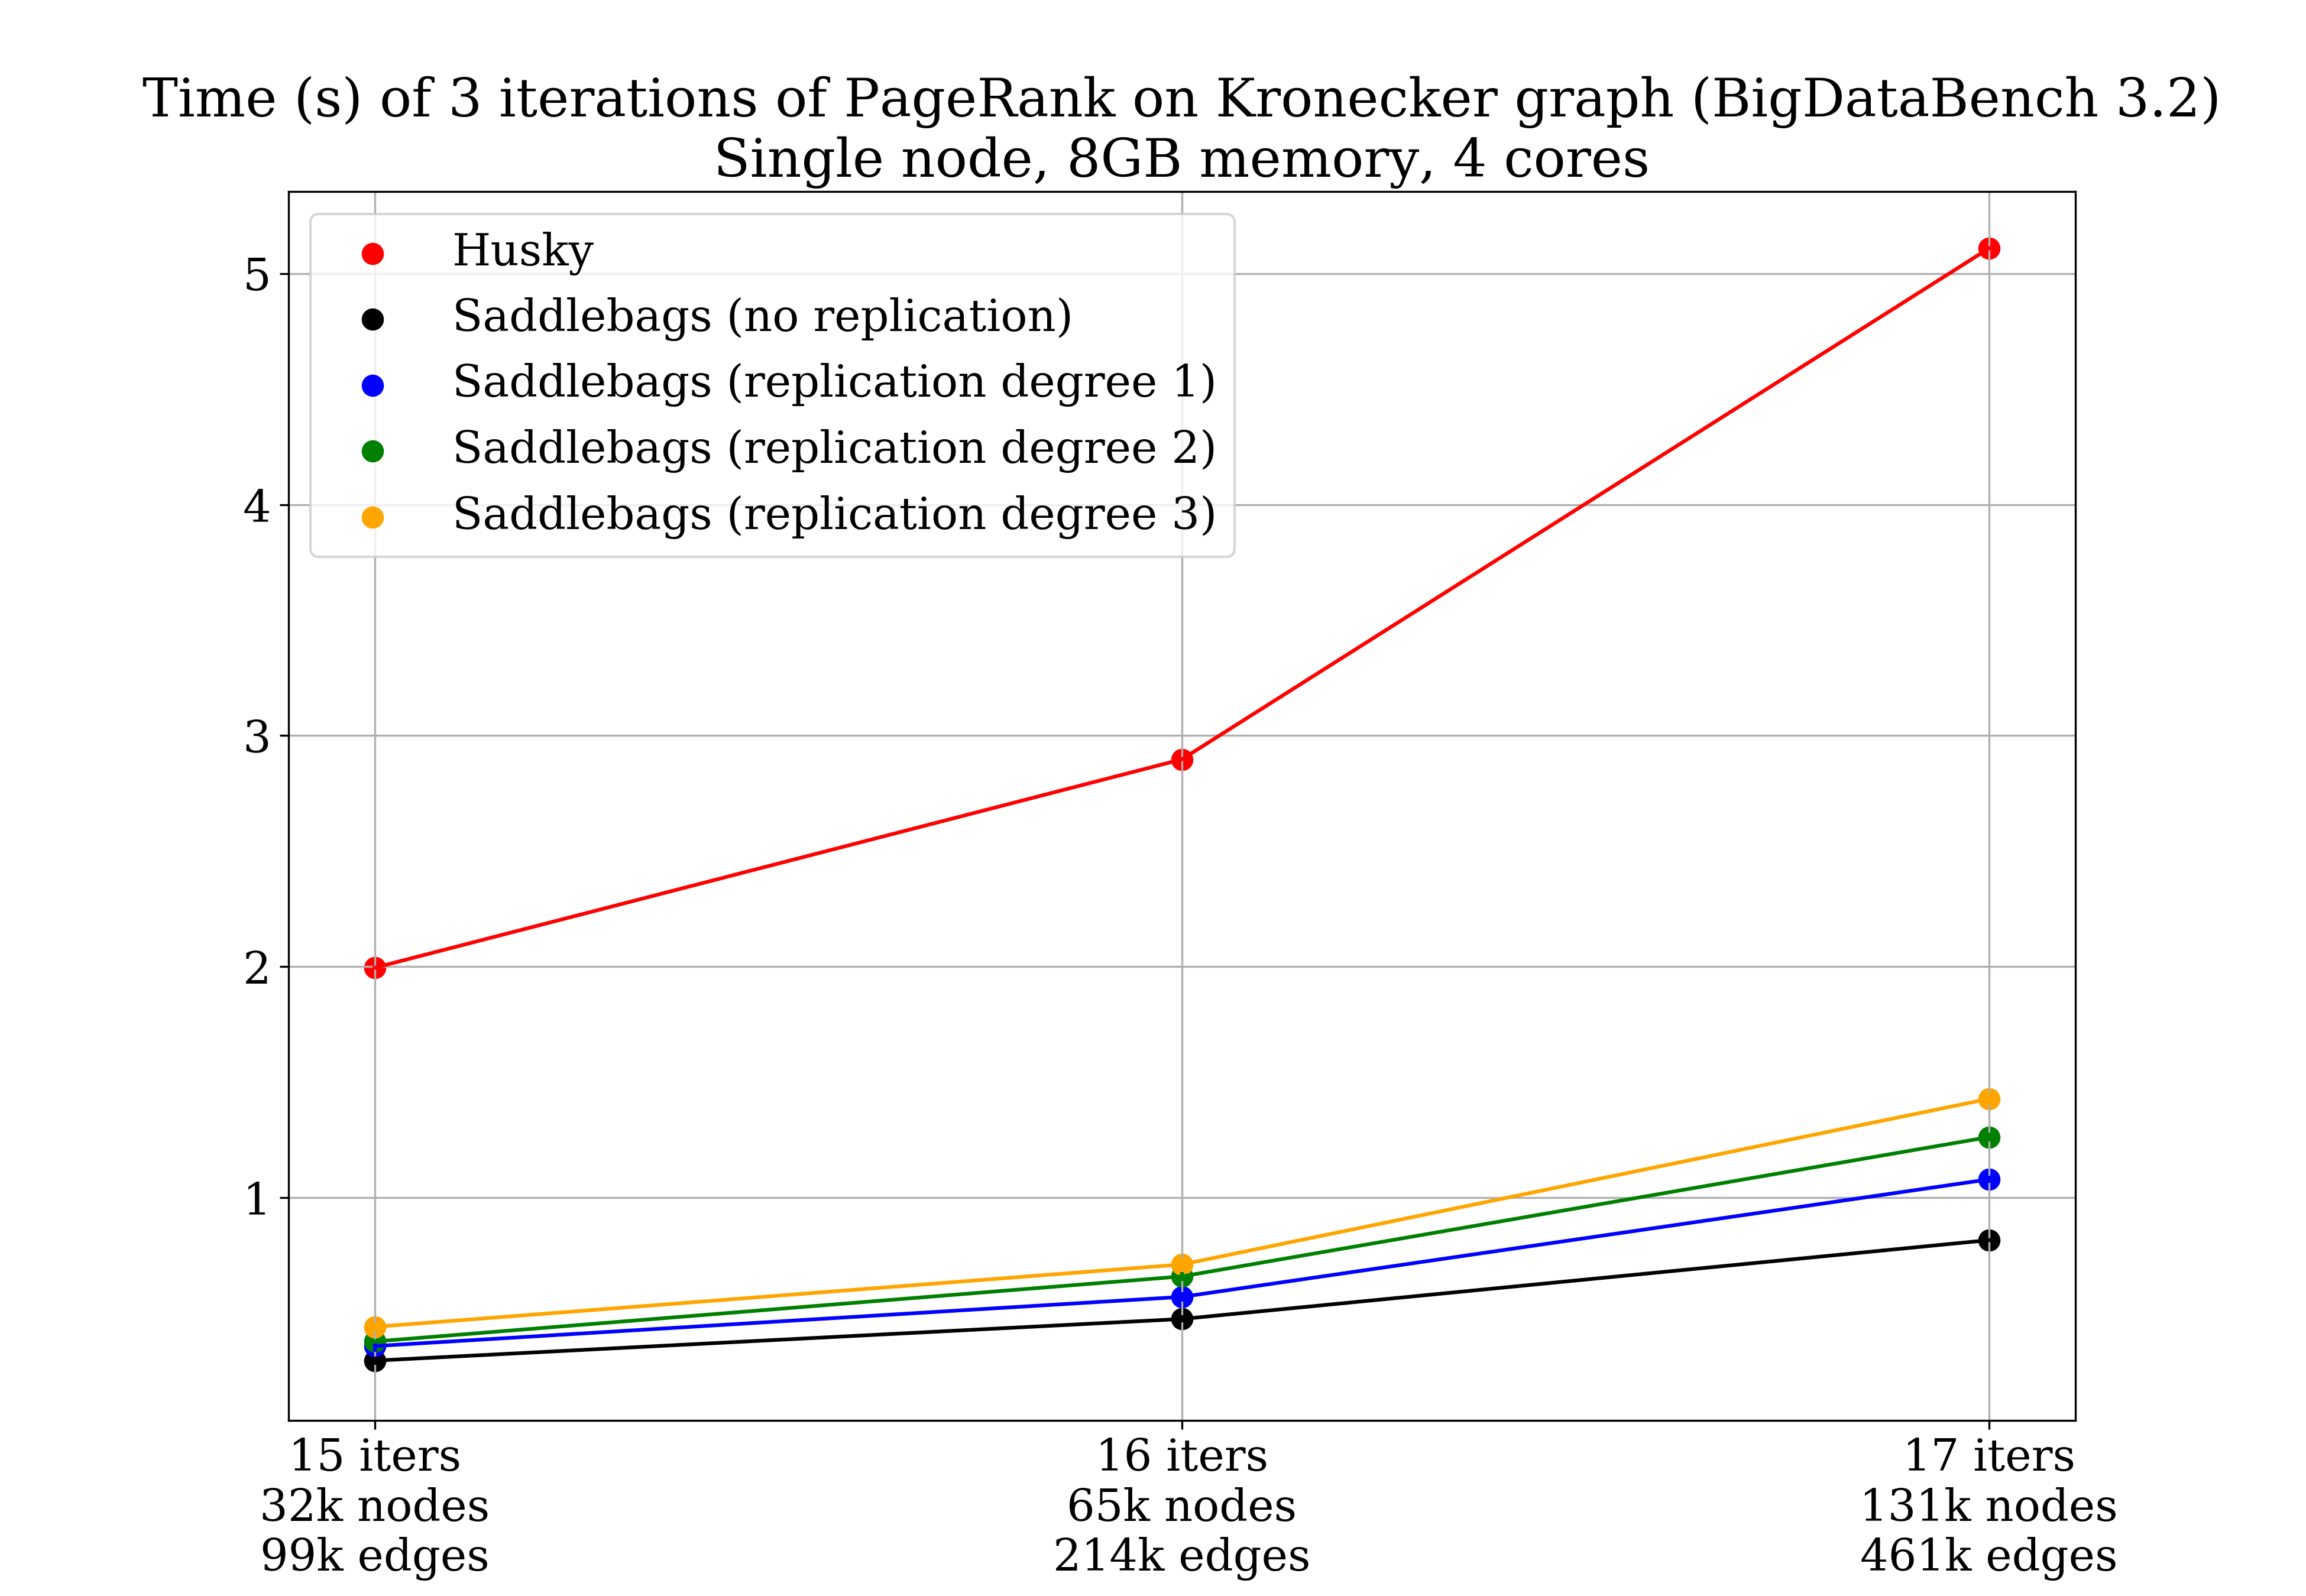
\includegraphics[width=15cm]{illustrations/png/replication.png}
	\caption{Execution time of PageRank in Saddlebags with replication}
	\label{fig:huskyfaulttolerance}
\end{figure}

\newpage
\section{Internal configuration} \label{section:configuration}
\subsection{Message ordering}
Parts of the TF-IDF experiment from section \ref{section:sparkeval} was performed again with ordered pulls enabled. Normally, in the Saddlebags implementation of TF-IDF, the item for every unique word that occurs in a document will perform two pull operations. For this experiment, the number of pulls per item was increased to 30. Ensuring that pulls are returned in the same order as they were sent in serves no purpose in TF-IDF, and the extra pull messages implemented for this experiment are extraneous. This was done only to observe performance differences when messages are delivered in-order. Figure \ref{fig:ordering} shows the results of this experiment. While the average execution time of the program with ordered messages was higher, both results are within the area denoted by each other's standard deviation. The difference in implementation is that ordered messages contain a sequence number integer, and that an indexed O(1) lookup of the messaging buffer is performed when storing the returned message, as opposed to always storing it at the end of the buffer. It is possible that, for problems with a certain degree of computational intensity, the complexity of message ordering is insignificant.
\vskip 0.5cm
\begin{figure}[H]
	\centering
	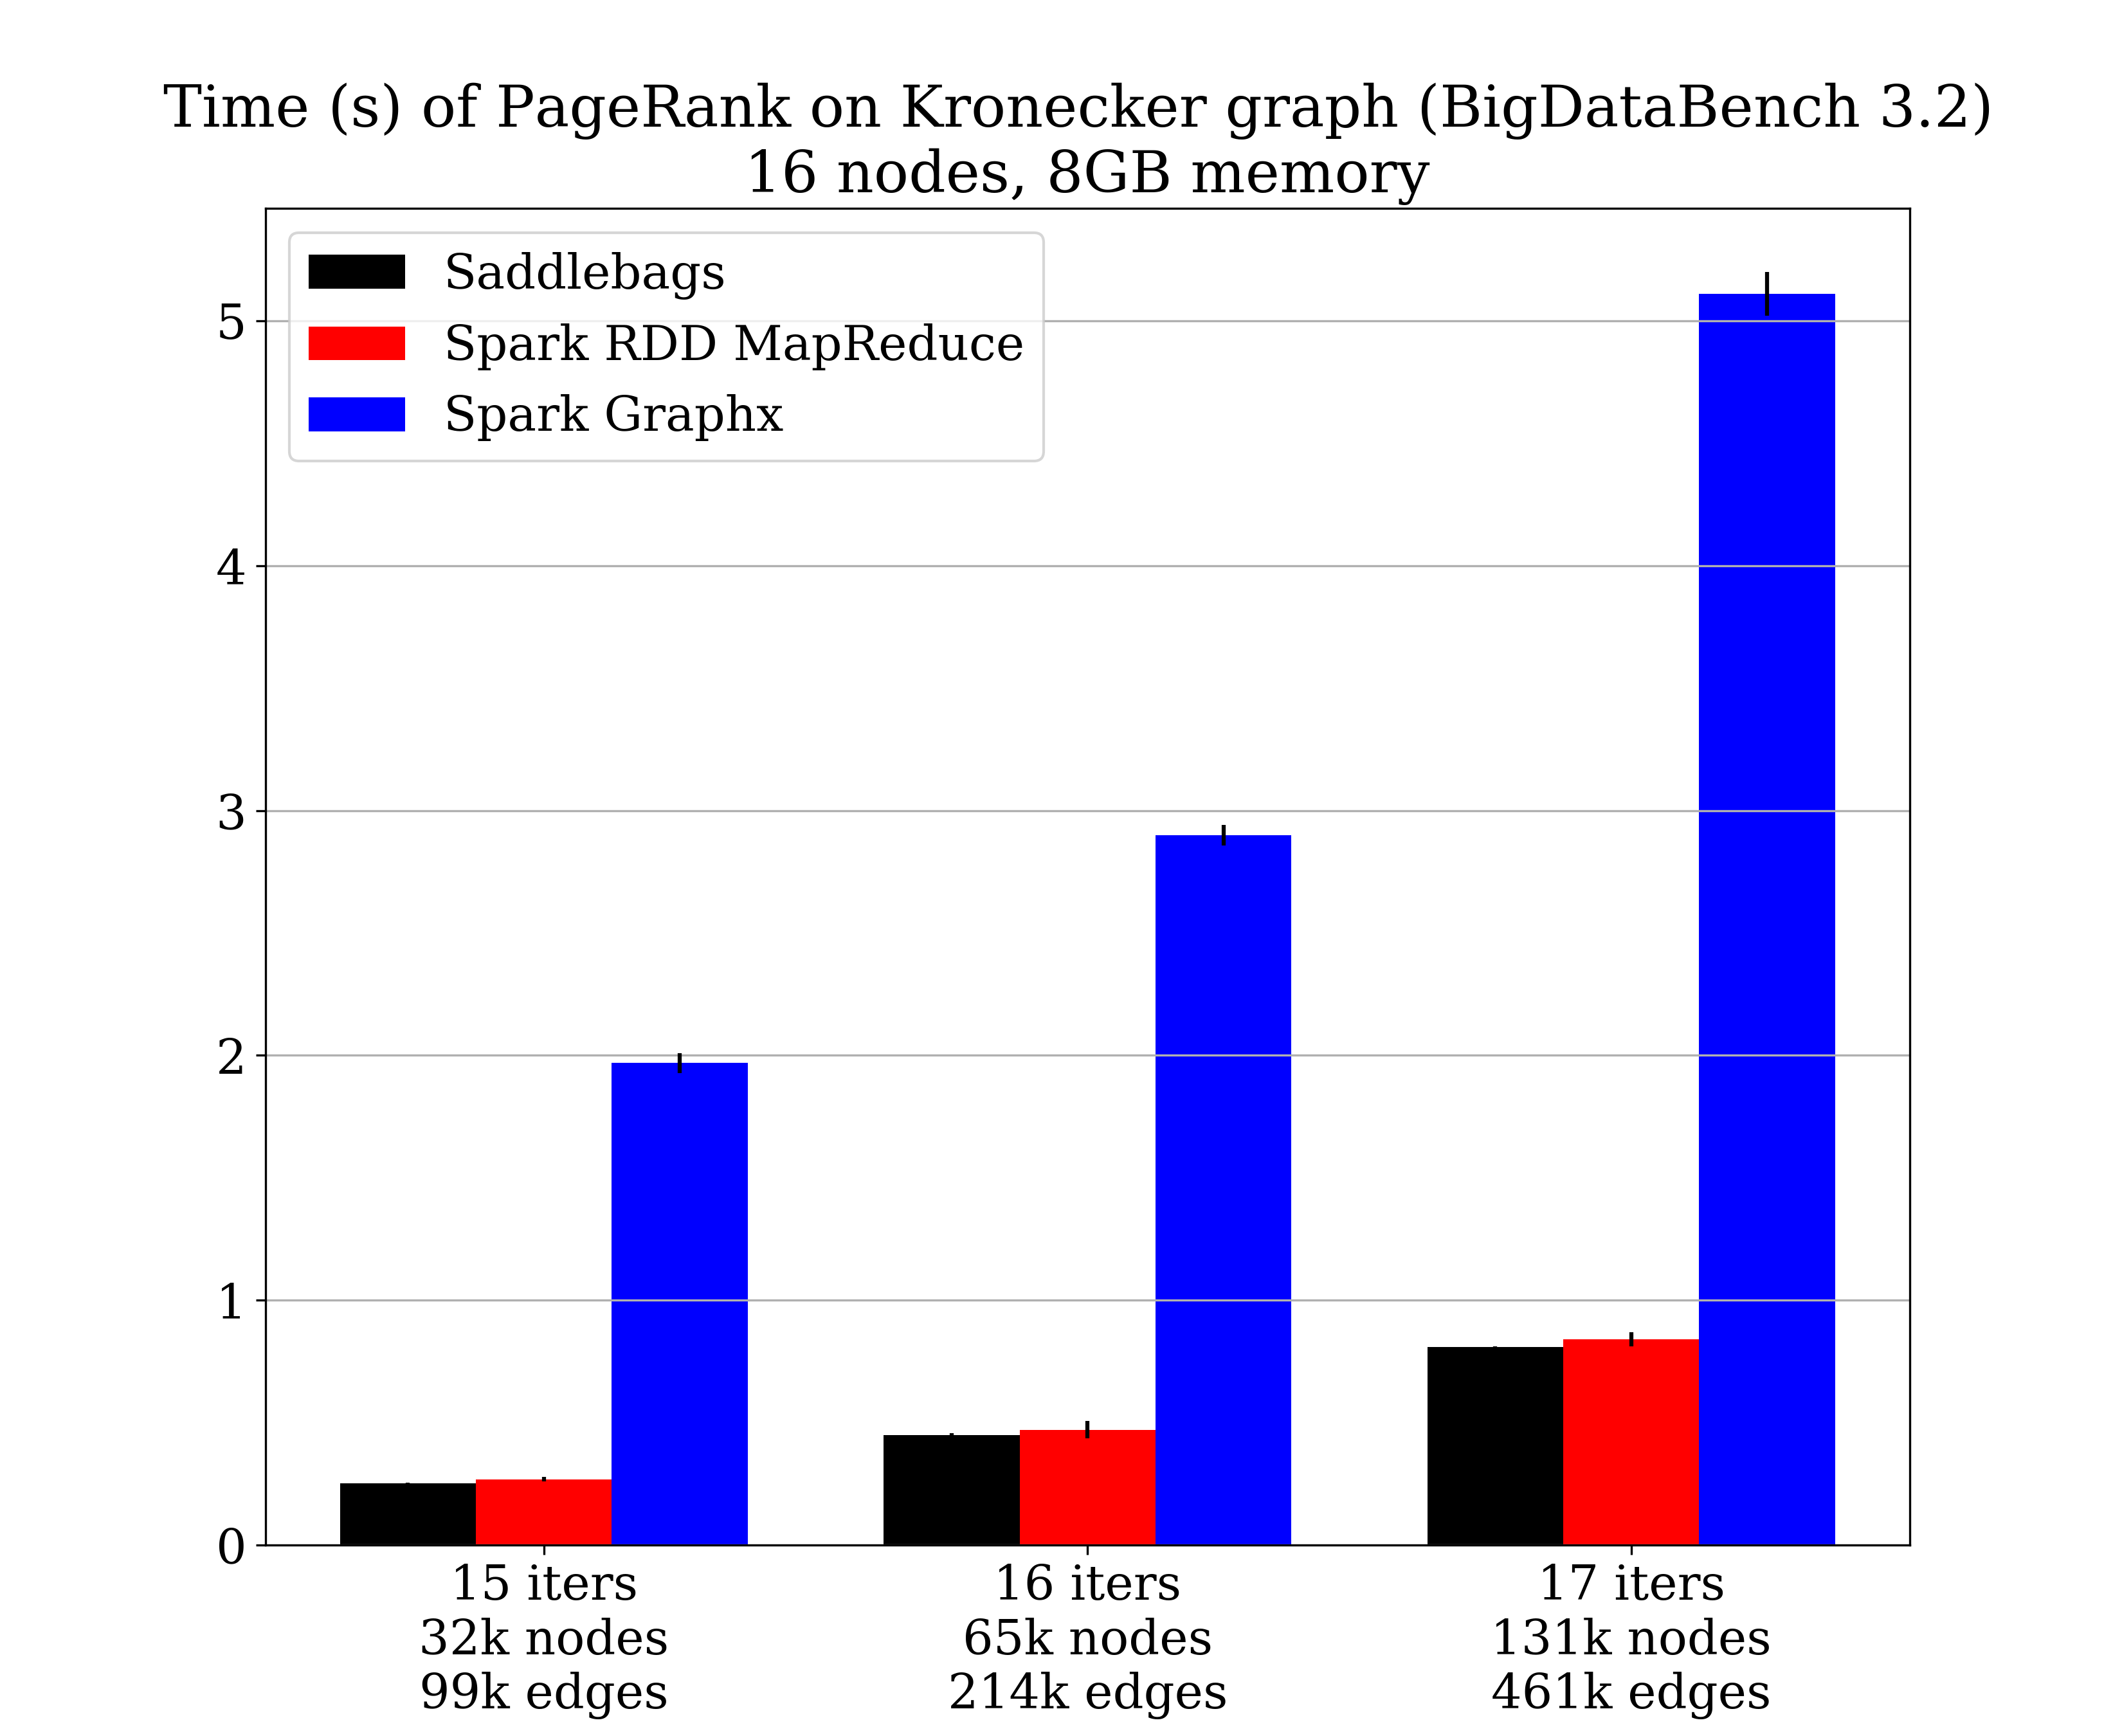
\includegraphics[width=13cm]{illustrations/png/messageordering.png}
	\caption{Execution time of TF-IDF with ordered pulls}
	\label{fig:ordering}
\end{figure}
\newpage
\subsection{Sending modes} \label{section:sendingmodeseval}
Different sending modes were outlined in section \ref{section:sendingmodes}. The PageRank benchmark was ran with different sending modes to investigate their performance implications. This benchmark was performed on the 16 core server and the cluster with 16 nodes. Both systems were included because of how UPC++ and GASNet communication implementation differs from single nodes and distributed systems. On the server, communication is achieved through shared memory. On the cluster, communication is achieved through message passing over InfiniBand.

Figure \ref{fig:sendingmodes} shows results from benchmarks on the server. In this environment, \\\texttt{GasnetBuffering} showed the worst performance. This sending mode avoids the Message abstraction, and achieves bulk synchronous parallel behavior by ignoring incoming RPCs until all local work has been completed. \texttt{Direct}, which also avoids the Message abstraction but handled RPCs immediately and disables bulk synchronous parallel behavior, showed the best performance, similar to \texttt{Buffering}. Figure \ref{fig:sendingmodesabel} shows results from benchmarks on the cluster. Here, \texttt{Combining} showed the best performance by a significant margin, followed by \texttt{GasnetBuffering}. \texttt{Buffering} and \texttt{Direct} showed similar performance.

It is clear from these results that combining messages to reduce communication overhead is an effective technique in cluster environments. On single nodes, where communication is not executed through message passing, combining seems to have little effect, and may be unbeneficial because of the complexity introduced by the combination functionality.
It can also be observed that \texttt{Buffering} is less performant than avoiding the Message abstraction on the cluster. The poor performance of \texttt{GASNetBuffering} on the single node is also notable. It has been claimed that, due to caching issues, UPC++ programs will execute sub-optimally when few \texttt{progress}-calls are made \cite{gasneteventissues}, which is the case for \texttt{GASNetBuffering}. This behavior varying between single nodes and cluster environments would explain differences in observed results of \texttt{GASNetBuffering} and \texttt{Buffering} between the two.



\newpage
\begin{figure}[H]
	\centering
	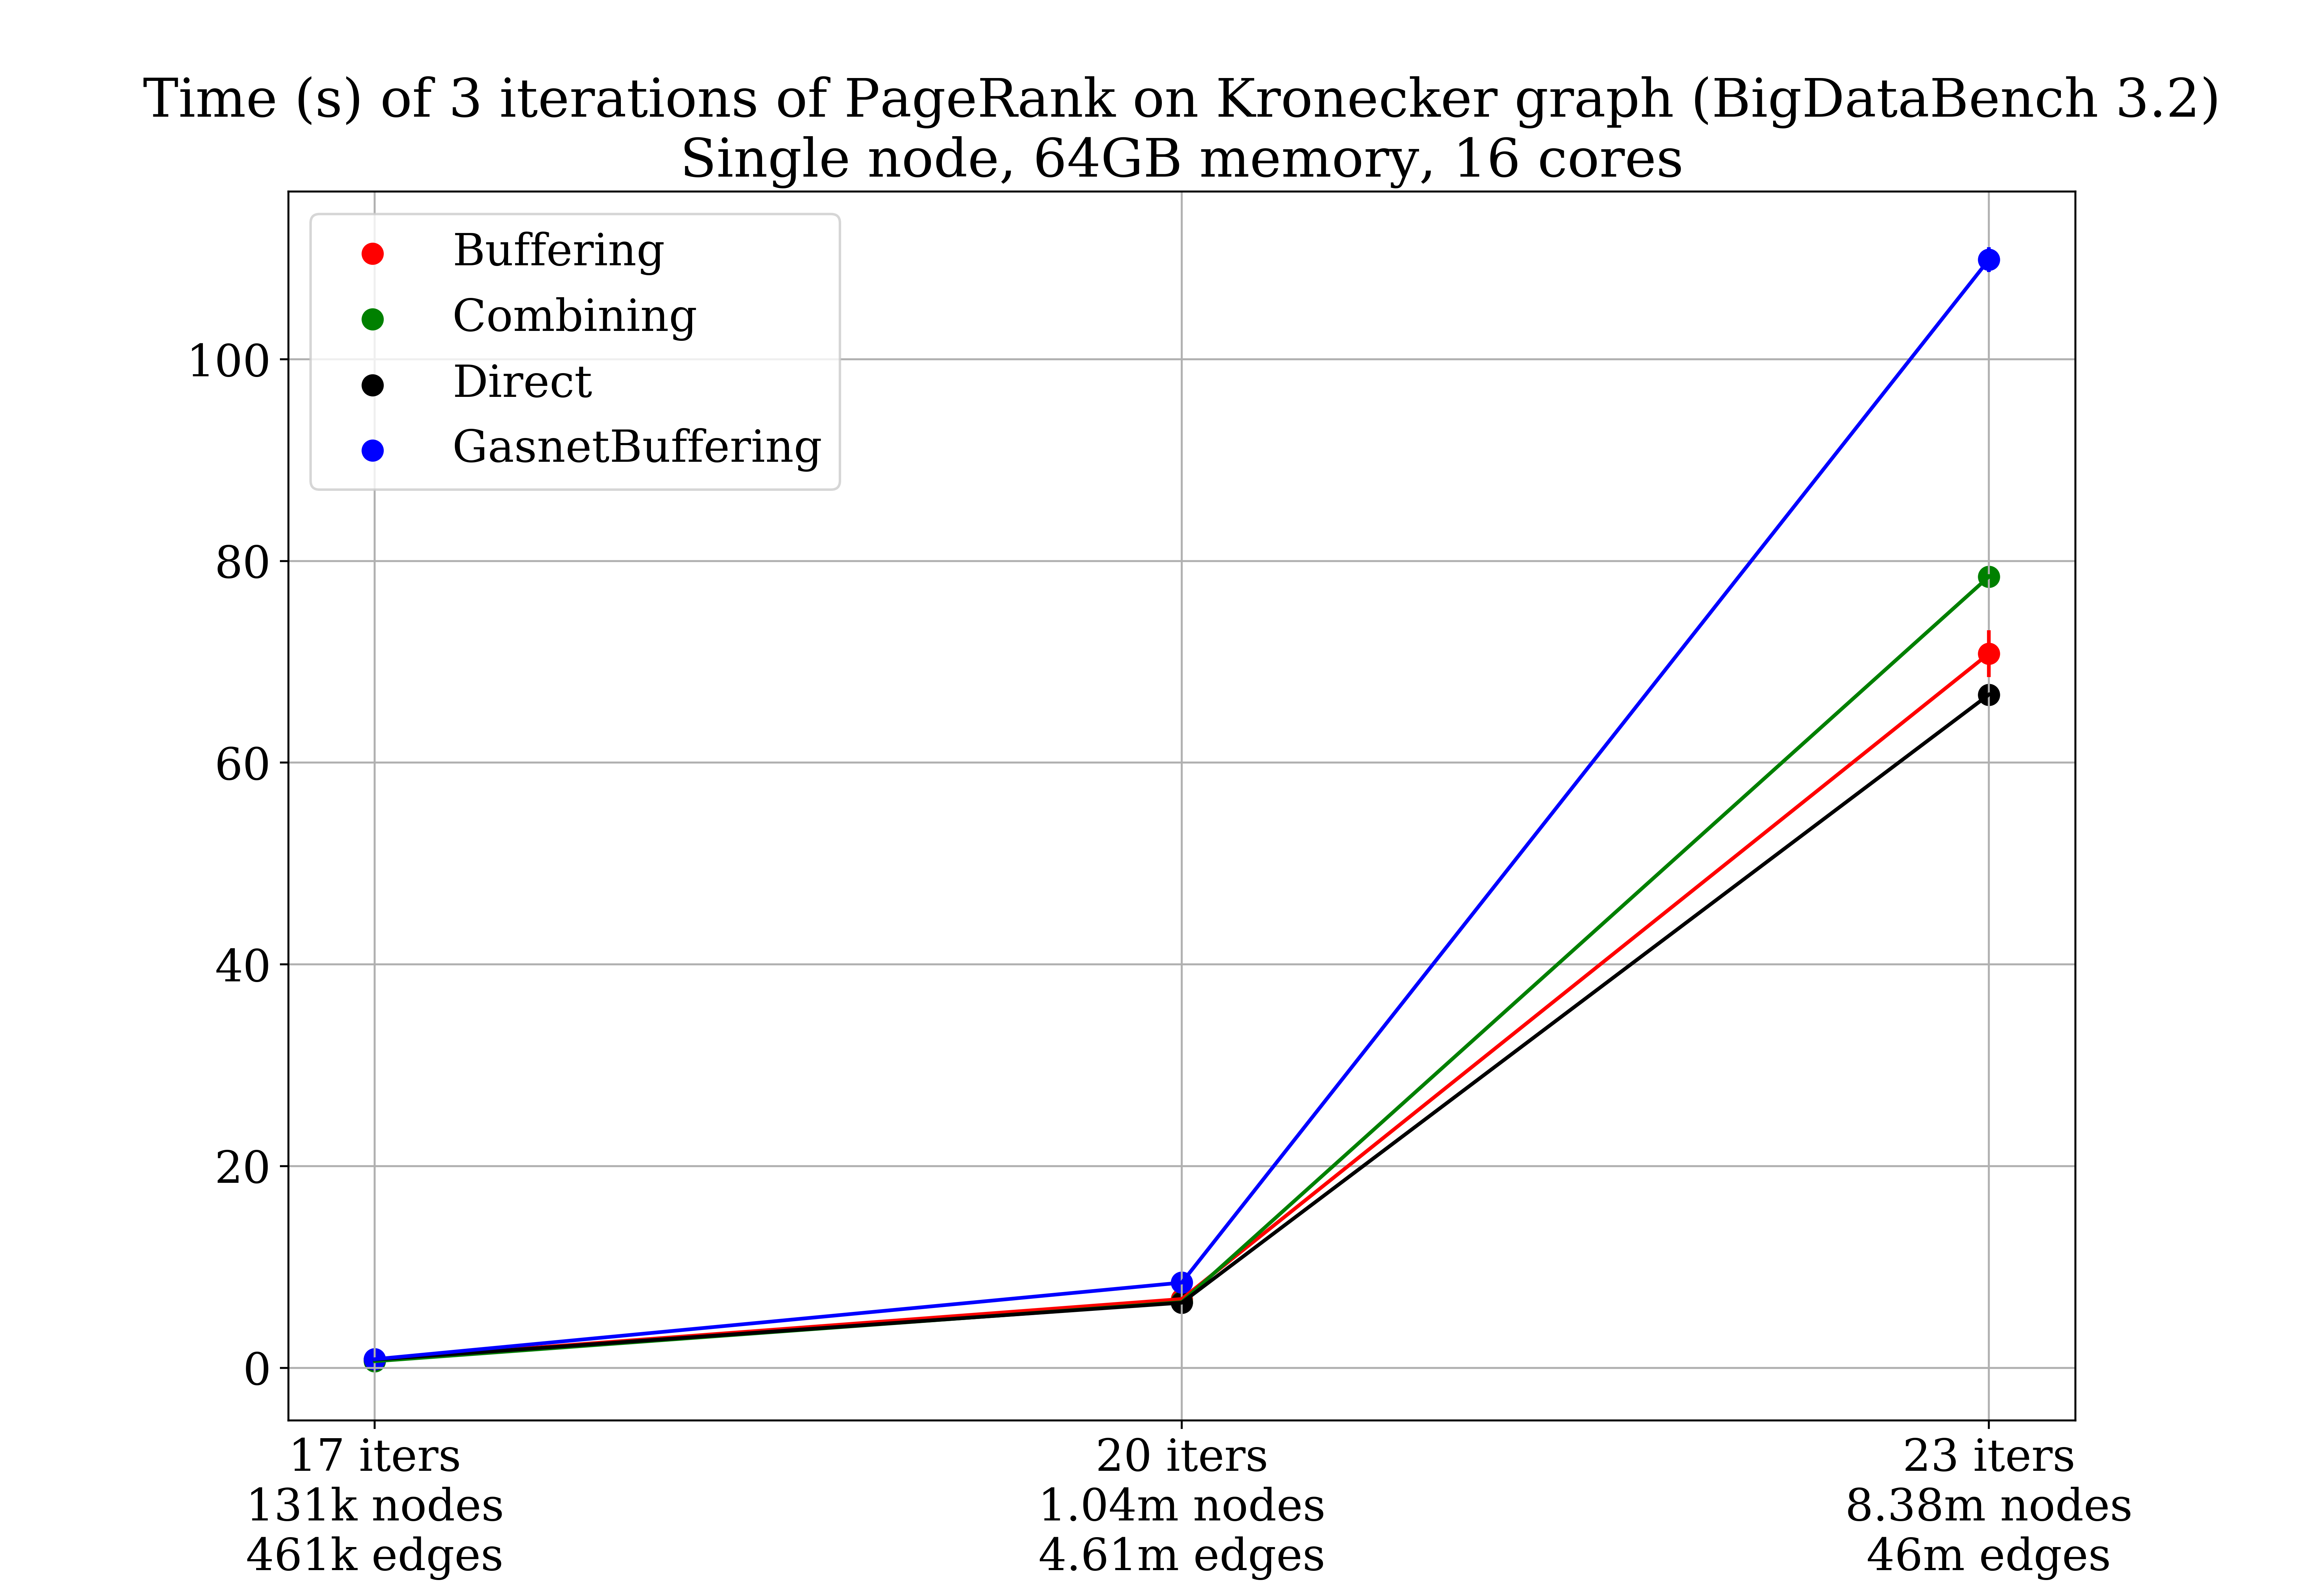
\includegraphics[width=15cm]{illustrations/png/sendingmodessinglenode.png}
	\caption{Execution time with different sending modes, single node}
	\label{fig:sendingmodes}
\end{figure}

\begin{figure}[H]
	\centering
	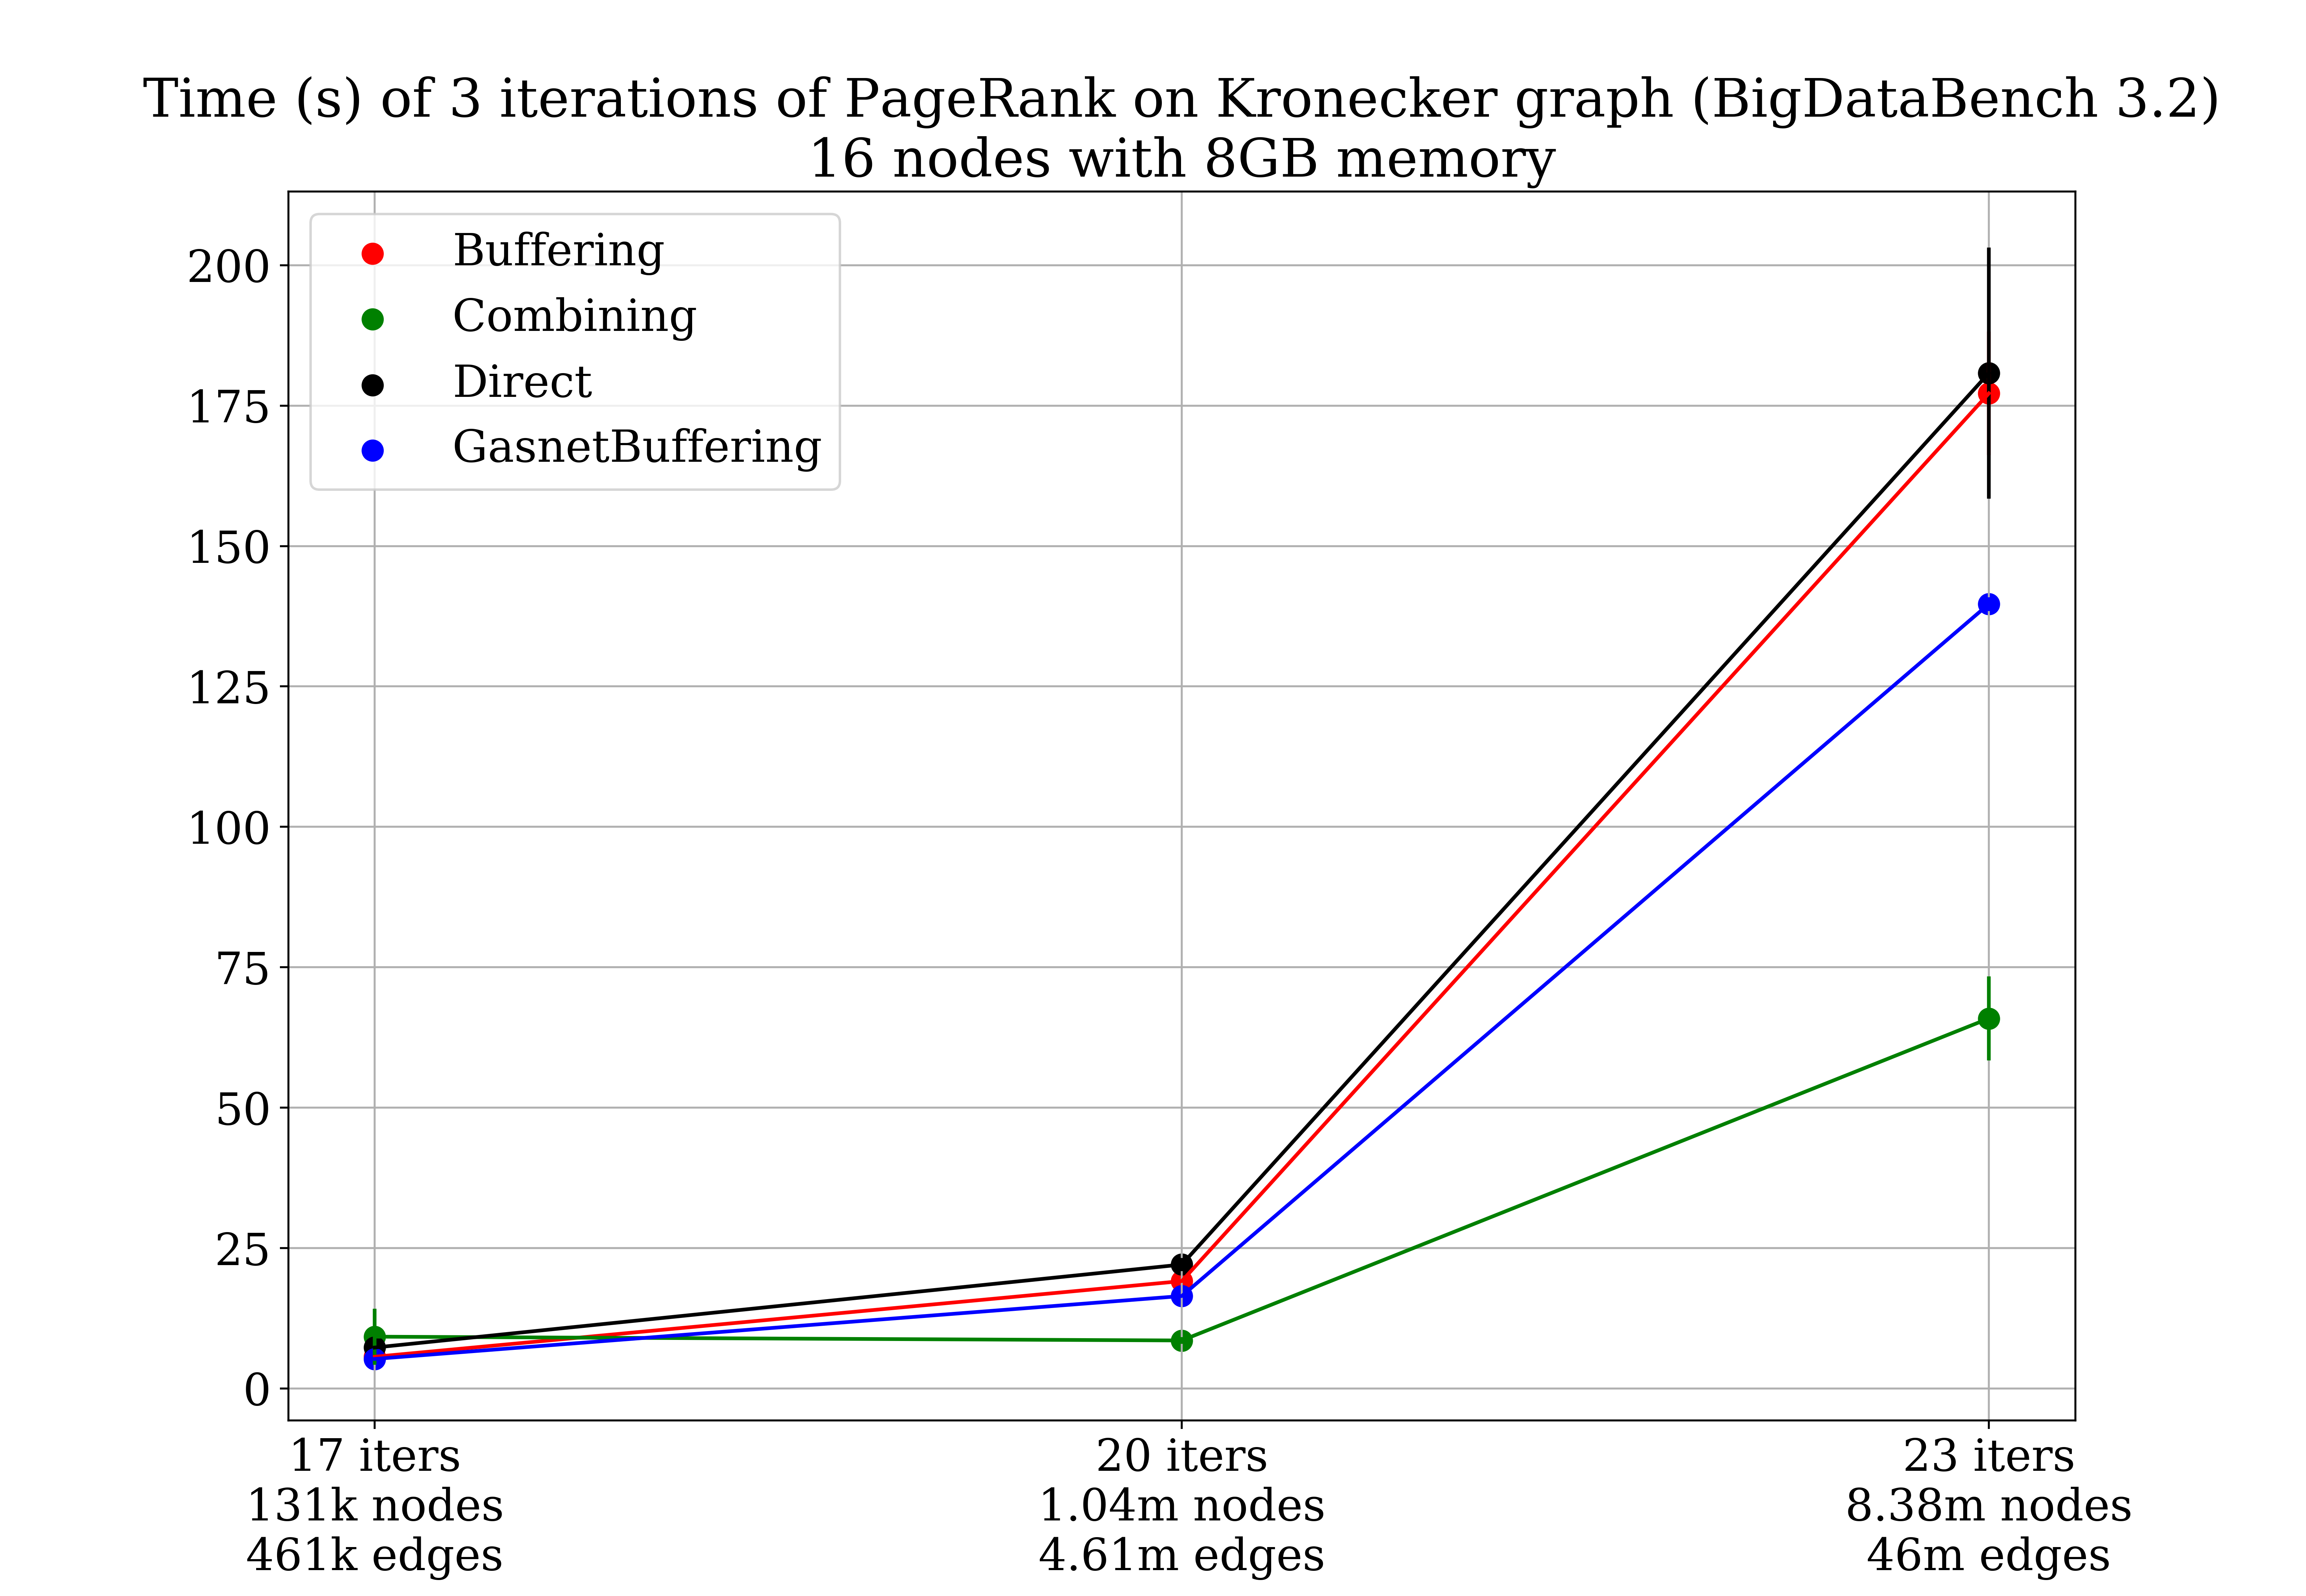
\includegraphics[width=15cm]{illustrations/png/sendingmodescluster.png}
	\caption{Execution time with different sending modes, cluster}
	\label{fig:sendingmodesabel}
\end{figure}


%\section{Energy efficiency}
%\section{Abstraction costs}
%\section{Comparison with other systems}
\newpage
\mbox{} \pagebreak
\newpage
\chapter{Discussion and Future Work} \label{section:discussion}
This chapter will provide a discussion on the findings from the previous chapter, and provide an outline of potential extensions and improvements that can be made to Saddlebags.

\section{Benchmark selection}
PageRank and TF-IDF were chosen as benchmarks because they are used prominently in the Husky paper, and because they represent different workload characteristics, namely a graph computation and a data intensive computation. Implementations of these problems were also widely available as example programs for Spark and GraphX. While these benchmarks showed results in favor of Saddlebags, it is difficult to proclaim its prominence as a general purpose HPC framework, since a larger and more varied set of problems is relevant in this field. In terms of throughput, it is naturally not possible to evaluate every existing HPC problem. In terms of programmability, universal classifiers such as Turing completeness checks are insignificant since Saddlebags applications are already implemented in the general purpose programming language C++. 

A systematic approach to evaluating parallel programming systems was taken by Asanovic et al. \cite{dwarfs}, where 13 \emph{dwarfs} (often referred to as \emph{Berkeley Dwarfs}) are used in place of traditional benchmarks. A dwarf is an algorithm or mathematical problem that captures a pattern of computation and data movement that constitutes a classification of problems with similar workload characteristics. 7 of the 13 Berkeley dwarfs were devised by Colella \cite{colella} in 2004 as numerical methods of importance in science and engineering. Inspired by these, Gao et al. \cite{datadwarfs} defined 8 dwarfs found in big data analysis applications. All of these dwarfs are listed in table \ref{table:dwarfs}. There is some overlap between the classes of dwarfs.

Example applications are given for each big data analysis dwarf. TF-IDF fits into this taxonomy as part of the Statistic Operations class. PageRank fits into the classes of Sampling and Graph Operations.

\vskip 0.9cm
\begin{table}[h]
	\begin{center}
		
		\setlength\arrayrulewidth{1pt}
		\renewcommand{\arraystretch}{2}
		\begin{tabular}{ | p{4cm} | p{4cm} | p{4cm} |}
			\hline
			\textbf{Numerical} & \textbf{Berkeley} & \textbf{Big data}\\ \hline
			Dense linear algebra & Combinational logic & Linear algebra \\ \hline
			Sparse linear algebra & Graph traversal &  Sampling \\ \hline
			Spectral methods & Dynamic programming &  Logic operations \\ \hline
			N-Body Methods & Backtrack and branch+bound &  Transform operations \\ \hline
			Structured Grids & Construct Graphical Models &  Set operations \\ \hline
			Unstructured Grids & Finite State Machine &  Graph operations \\ \hline
			Monte Carlo/MapReduce &  &  Sorting algorithms\\ \hline
			 &  &  Statistic operations\\ \hline
		\end{tabular}
		\caption{Dwarf classifications}
		\label{table:dwarfs}
		
	\end{center}
\end{table}






\newpage
Example applications have been implemented in Saddlebags for sequential and distributed dense matrix multiplication. Set operations such as union, intersection and complement, can be implemented on a per-application basis, using table lookups and distribution schemes. Saddlebags can be extended to support this natively. The remaining big data dwarfs, Logic Operations (described as a collection of hash algorithms) and Sort classifications, have not been investigated. Considering the unordered nature of Saddlebags tables, implementing sorting algorithms with items will likely be unintuitive.

Section \ref{section:programmability} investigated the programmability of Saddlebags in comparison with Husky and Pregel. These systems are natural targets for comparison as they provide a similar programming model, and it is often possible to find clear one to one relationships between different parts of their implementations. For example, vertices have clearly defined algorithm iteration tasks and communication routines, as shown in table \ref{table:programmability}. This enables detailed comparisons of frameworks, and implementation details and features such as data distribution, message protocols and code organization can be investigated. From a user-perspective, an overview like this is useful when deciding between frameworks that implement a similar programming model. However, it does not say much about the usefulness of this particular class of frameworks. For this, a more structured view of HPC and big data problems is required. For a more convincing performance evaluation and showing of expressiveness, more of the big data and Berkeley dwarfs should be provided. This is advantageous both for benchmarking a larger array of problems, and for examining the programmability of Saddlebags and other frameworks with similar programming models. 

Providing implementations and benchmarks for problems of every dwarf classification will be complex and time consuming work, but it can be argued that such a collection of solved HPC problems is required before proclaiming that a framework suits a purpose more general than solving select problems. If the goal is to provide a unified HPC and big data framework, implementing workloads from all 13 Berkeley dwarfs and all 8 big data analysis dwarfs is an opportunity to demonstrate a framework's viability in both fields. Disregarding performance, an evaluation of the programming model of Husky or Pregel in context of the dwarfs would likely be relevant for Saddlebags as well. For an experiment like this, it would be assumed that problems that can be implemented in one of these frameworks could also be implemented in Saddlebags. However, no overview of Berkeley dwarf implementations in these frameworks have been found; Pregel is classified as a graph analysis framework and such a comparison is likely out of its scope, and Husky relies on performance benchmarks of different workload types rather than dwarf classifications. In addition to the workloads already demonstrated, Husky shows that their programming model is suitable for various machine learning tasks.

%If we were to dis

\section{Variants of fault tolerance}
Fault tolerance is provided in Saddlebags, by replicating data throughout partitions. This is a technique adopted by different storage systems \cite{dynamo, ramcloud, chord}, and has the advantage of keeping all data in memory, which avoids the inherent slowdown of accessing persistent storage. Other fault tolerance systems involve periodically storing data or program state to disk, a process that is slower but allows recovery at the same node rather than moving computation to a different node.

Spark's RDD transformation execution model allows for recreation of data, since all operations can be logged inexpensively compared with fine-grained memory access models. This approach to fault tolerance is a fundamental part of the framework; replication and checkpointing approaches of other systems can be disabled or customized for higher throughput, but Spark's RDDs are designed around its fault tolerance model. Performance evaluations such as those presented in section \ref{section:sparkeval} may give the impression that the coarse grained operation model adopted by Spark is strictly worse than fine grained access, but the execution model also provides durability, which is not reflected in benchmark results. 

Saddlebags' fault tolerance model is designed for high performance, with customizable replication level for transparent data movement. Should one require guarantees for crash recovery, other frameworks would be more suitable. While Spark provides an absolute guarantee of fault tolerance, and many traditional HPC frameworks ignores fault tolerance altogether, Saddlebags aims for a compromise. Should Saddlebags aim to provide more robust fault tolerance, it would implement checkpointing to disk in Young/Daly periods, which is the modern standard for fault tolerance within HPC~\cite{herault2016fault}.

\section{Message types}
The messaging model that has been described in this thesis assumes that a single type, passed as a template parameter to a worker, is the only data type that can be used for communication. Section \ref{section:programmability} showed that Husky allows more flexible message passing, while Pregel also restricts messaging to a single type. While this is a restriction to programmability, some approaches can be taken to achieve a more flexible system. 

The C++ boost library provides a class \texttt{any} \cite{boostany} that can hold data of different types. The responsibility of identifying different types within this class in messages is left to the user when type is used.

UPC++ global pointers, as described in section \ref{section:globalpointers}, can be used as messaging types, so that items are sending pointers to a shared memory segment in its messages. This allows for data of any structure to be communicated across items. This increases implementation complexity of the \texttt{Item} class, as synchronization of accessing data from global pointers is left up to the user.

%global pointers
%boost any

%\section{Possible extensions}

\section{UPC++ versions}
Saddlebags was implemented and tested with UPC++ version 2017.9.0. At the time of this writing, two more recent versions has been released, 2018.1.0 and 2018.3.0. Some features of these versions could provide improvements to Saddlebags.

\subsection{Shared heap size}
A recent feature of significance is that of a parameter that allows customization of shared heap size. This means that the maximum size allocated to shared memory segments, which contain global pointers and RPC data, can be tuned before executing a UPC++ program. The replication test in section \ref{section:replicationeval} was only performed on a single node, as the cluster nodes ran out of memory allocated to the shared segment due to the memory cost of replication, and the differing communication models applied on clusters and single node systems. Since the program is implemented in an earlier version of UPC++, the shared heap size can not be configured at this time, and is fixed at 128 MB \cite{upcxxguide20183}. For this reason, the largest focus of future work on Saddlebags should be porting it to a more recent version of UPC++. Possible compatibility-breaking features of new releases would make this effort only worthwhile when useful features or fixes are released, such as shared heap size customization.


\subsection{View-based serialization}
UPC++ version 2018.3.0, released March 2018, introduced an alternative serialization model for transmitting collections of objects via RPCs, named view-based serialization. Prior to this update, transmission of an arbitrarily count of objects was done through explicitly packaging objects into containers such as the C++ standard library \texttt{vector} type. In Saddlebags, both transmission of data for replication and the \texttt{Combining} sending mode are implemented in this fashion. View-based serialization can be used as an optimization through the \texttt{View} type, which provides an iterator that traverses items in the network buffer used for RPCs \cite{upcxxguide20183}. The significance of this technique is that it avoids the creation and teardown of containers such as vectors that hold no additional information other than the collection of objects.

It was shown in section \ref{section:sendingmodeseval} that \texttt{Combining} is the preferred sending mode for cluster environments, and improving this sending mode is a possible area of focus for improving the performance of Saddlebags. Due to its debut in the 2018.3 version of UPC++, view-based serialization has not been utilized in this release of Saddlebags.


%\subsection{File input}
%input of file formats?
%input of filled-out tables, like how rdds can be stored to disk and loaded

%other features from spark


\chapter{Conclusion}
This thesis has presented Saddlebags, a High Performance Computing framework implemented in C++, using the UPC++ library for a partitioned global address space communication model. Saddlebags aims to provide support for workloads from the fields of both HPC and big data analysis. This is achieved by providing features from big data analysis that allows for easier programming and handling of large volumes of data, while providing a lightweight and customizable execution model. Inspired by big data systems, Saddlebags provides implicit distribution of data, moves computing tasks to the location of its data, provides fault tolerance, and relieves programmers of implementing specialized communication routines and synchronization. Additionally, all data movement and communication is explicit, and data can be remotely accessed in fine-grained fashion.

Saddlebags implements a bulk synchronous parallel programming model that is inspired by graph computing frameworks, but aims to support more diverse workloads. Saddlebags programs are based around extending a general-purpose data item class, that is accessible from all parallel partitions through RPCs. This base item class provides communication features and can be extended to execute computational tasks. Like UPC++, Saddlebags is customizable through C++ template programming.

Fault tolerance is implemented with customizable in-memory replication techniques that has previously been used in various storage systems, in order to avoid the slowdown of accessing persistent storage. Several protocols for messaging between concurrent partitions have been implemented, with different performance characteristics and use-cases for programs running on individual nodes and compute clusters.

Benchmarks shows that this approach, coupled with a communication layer implementation by UPC++ and GASNet, provides favorable performance in comparison with other contemporary systems for HPC and big data analysis. What is left for the future is a more extensive investigation of the various classifications of workloads that can benefit from the Saddlebags programming model.

\pagebreak
\bibliographystyle{ieeetr}
\bibliography{thesis}
\newpage
\mbox{} \pagebreak
\appendix
\chapter{Installing and using Saddlebags}
This section will explain how to install UPC++, and use Saddlebags on different platforms. All compute clusters with InfiniBand or Ethernet connections that support MPI is expected to work, but this section will focus on major Norwegian HPC infrastructure, namely the Abel cluster at University of Oslo, and the Stallo cluster, at the University of Tromsø. Installation instructions are available in the UPC++ implementation tarball, and are also included here to provide specific instructions for modules and workload managers found in Norwegian university clusters. An overview of the included Saddlebags applications is provided in a readme file in the source code.

Saddlebags has been implemented and tested with UPC++ v2017.9.0, which can be found at {\url{https://bitbucket.org/upcxx/upcxx/downloads/upcxx-2017.9.0.tar.gz}}.
\section{Linux installation}\label{section:installinux}
Unzip the tarball, and run the \texttt{install} file, with installation directory as argument:\\
\phantom{11111} \texttt{\$ ./install /desired/installation/directory}\\
Store the installation directory in an environment variable\\
\phantom{11111} \texttt{\$ export UPCXX\_INSTALL=/desired/installation/directory}\\
\subsection{Running UPC++ programs on Linux}\label{section:runlinux}
First, set a memory limit per node.\\
\phantom{11111} \texttt{\$ export GASNET\_PHYSMEM\_MAX='8000MB'}\\



There are two ways of running a UPC++ programs in a non-distributed environment. The first method involves setting the number of partitions in an environment variable, and running the program normally.\\
\phantom{11111} \texttt{\$ cd upcxx-2018.1.0/example/prog-guide}\\
\phantom{11111} \texttt{\$ make}\\
\phantom{11111} \texttt{\$ export GASNET\_PSHM\_NODES=4}\\
\phantom{11111} \texttt{\$ ./hello-world}\\

Another method is using the \texttt{upcxx\_run} script in the install location, with the number of partitions as argument.\\
\phantom{11111} \texttt{\$ \$UPCXX\_INSTALL/bin/upcxx-run 4 hello-world}\\

The default communication conduit is detected during installation. It can also be set manually.

InfiniBand (clusters):\\
\phantom{11111} \texttt{\$ export UPCXX\_GASNET\_CONDUIT=ibv}\\
Shared memory (single node):\\
\phantom{11111} \texttt{\$ export UPCXX\_GASNET\_CONDUIT=smp}\\
MPI:\\
\phantom{11111} \texttt{\$ export UPCXX\_GASNET\_CONDUIT=mpi}\\

Saddlebags applications are compiled with the \texttt{make} command. Note that for Abel, the \texttt{mpicxx} C++ compiler must be used.
\subsection{Abel}
Abel uses the Lmod environment module system. Before installation can be performed as in the previous section, the proper modules must be loaded. \\
\phantom{11111} \texttt{\$ module purge}\\
\phantom{11111} \texttt{\$ module load python2/2.7.10.gnu}\\
\phantom{11111} \texttt{\$ module load gcc/7.2.0}\\
\phantom{11111} \texttt{\$ module load openmpi.gnu/2.1.0}  \\
First, any pre-loaded modules are removed to ensure that the intended compiler is used. MPI is needed for communication between nodes, and thread spawning. Python is needed for installation 

With all modules loaded, follow the normal Linux installation instructions found earlier in this section. Programs are compiled as shown in section \ref{section:runlinux}.

In order to run workloads on Abel, you need allocated CPU hours on a specific account name. To find your account name:\\
\phantom{11111} \texttt{\$ cost}\\
Run programs with the \texttt{salloc} command. Memory usage and max compute time must be provided:\\
\phantom{11111} \texttt{\$ salloc --nodes=16 --mem-per-cpu=8000 --time=01:00:00 --account=ACCNAME \$UPCXX\_INSTALL/bin/upcxx-run 16 ./hello-world}\\

\subsection{Stallo}
Stallo uses the same module system as Abel, but provides different default modules and names. Here, \texttt{mpicxx} can be set as the default C++ compiler during installation:
\phantom{11111} \texttt{\$ module load OpenMPI/2.1.1-GCC-6.4.0-2.28}\\
\phantom{11111} \texttt{\$ CC=mpicc CXX=mpicxx ./install /desired/installation/directory}\\
\phantom{11111} \texttt{\$ export UPCXX\_INSTALL=/desired/installation/directory}\\

Running programs on Stallo is similar as on Abel, but less information is required to queue workloads.\\
\phantom{11111} \texttt{\$ salloc --nodes=16 \$UPCXX\_INSTALL/bin/upcxx-run 16 ./hello-world}\\
Information about memory usage per node is not required, but should be added as an argument, like on Abel, if \texttt{GASNET\_PHYSMEM\_MAX} is set above 1 GB.


\chapter{API Reference}
This section will explain the API that can be used to implement programs in Saddlebags. Since template types in definitions, parameters, and return values, can make function signatures exorbitantly large, simplified versions are shown at first, with parameters and return types explained subsequently. Because classes can't hold references to themselves as distributed objects, many operations are implemented as functions rather than methods.
\vskip 0.6cm
\begin{center}
	\noindent\rule{4cm}{1.2pt}
\end{center}
\vskip 0.5cm
\textit{function} \texttt{create\_worker()}\\
\phantom{11111} Initializes and returns a Worker with the given template parameters, and the \texttt{Buffering} sending mode. It is returned as a UPC++ distributed object. \\
\textbf{Template arguments:}\\
\phantom{11111} \texttt{<class TableKey\_T, class ItemKey\_T, class message\_T>}\\
\textbf{Return type:}\\
\phantom{11111}  \texttt{upcxx::dist\_object< Worker<key\_T, value\_T, message\_T> >}\\
\textbf{Variations:}\\
\phantom{11111} \texttt{create\_worker(SendingMode mode)}\\
\phantom{11111}\phantom{11111} Returns a Worker with the given sending mode.

\newpage
\textit{function} \texttt{add\_table(worker, tableKey, is\_global)}\\
\phantom{11111} Adds a table to a worker. Template parameters indicate the Item type this table should contain, and the data distribution behavior this table should adopt.\\
\textbf{Arguments:}\\
\phantom{11111} \texttt{worker} - The Worker that a table will be added to\\
\phantom{11111} \texttt{tableKey} - The key that the table is indexed with in the Worker. The type of this parameter is given by the Worker's \texttt{TableKey\_T}\\
\phantom{11111} \texttt{is\_global} - Boolean. Whether the new table should be globally accessible

\textbf{Template arguments:}\\
\phantom{11111} \texttt{<class DistributorType, class ItemType>}\\
\textbf{Return type:}\\
\phantom{11111}  void\\
\textbf{Variations:}\\
\phantom{11111} \texttt{DistributorType} template argument can be ignored, to initialize a table with default hashing distribution logic.

\vskip 0.05cm
\begin{center}
	\noindent\rule{4cm}{1.2pt}
\end{center}
\vskip 0.15cm
\textit{function} \texttt{insert\_object(worker, tableKey, itemKey)}\\
\phantom{11111} Attempts to insert an object into a given table. If the table does not contain an item with the given key, a new item is created. If an item exists, its \texttt{refresh} method is called.  \\
\textbf{Arguments:}\\
\phantom{11111} \texttt{worker} - The Worker that contains the table the item should be inserted into\\
\phantom{11111} \texttt{tableKey} - The table that the item should be inserted into\\
\phantom{11111} \texttt{itemKey} - The key to associate the new item with\\
\textbf{Return type:}\\
\phantom{11111}  void\\
\textbf{Variations:}\\
\phantom{11111} \texttt{<ItemType\_T> ItemType\_T insert\_and\_return(worker, tableKey, itemKey)}\\
\phantom{11111}\phantom{11111} Given the item type as template parameter, the item that is referred to is returned.
\newpage

\textit{function} \texttt{lookup\_item(worker, tableKey, itemKey)}\\
\phantom{11111} A pointer to an Item is returned if it exists with the given key, in the given table, in the given Worker. Otherwise, \texttt{NULL} is returned.\\
\textbf{Arguments:}\\
\phantom{11111} \texttt{worker} - The Worker that contains the table to look for the item in\\
\phantom{11111} \texttt{tableKey} - The table that contains the item to look for\\
\phantom{11111} \texttt{itemKey} - The desired item\\
\textbf{Template arguments:}\\
\phantom{11111} \texttt{<class ItemType\_T>}\\
\phantom{11111}\phantom{11111} The type of the item\\
\textbf{Return type:}\\
\phantom{11111}  \texttt{ItemType\_T*}

\vskip 0.5cm
\begin{center}
	\noindent\rule{4cm}{1.2pt}
\end{center}
\vskip 0.7cm

\textit{function} \texttt{cycles(worker, num\_cycles)}\\
\phantom{11111} Perform the given amount of iterations in the Worker\\
\textbf{Arguments:}\\
\phantom{11111} \texttt{worker} - The Worker whos items should execute work\\
\phantom{11111} \texttt{num\_cycles} - The number of iterations to execute\\
\textbf{Return type:}\\
\phantom{11111}  void\\
\textbf{Variations:}\\
\phantom{11111} \texttt{cycle(worker, do\_work)}\\
\phantom{11111} \phantom{11111} Perform a single iteration. The second parameter is a boolean indicating whether work should be performed. If no work is performed, communication routines are still executed as in regular iterations.
\newpage


\textit{function} \texttt{iterate\_table(worker, table\_key)}\\
\phantom{11111} Get all items stored within a table\\
\textbf{Arguments:}\\
\phantom{11111} \texttt{worker} - The Worker containing the given table\\
\phantom{11111} \texttt{table\_key} - The table to get items from\\
\textbf{Template arguments:}\\
\phantom{11111} \texttt{<class ItemType\_T>}\\
\textbf{Return type:}\\
\phantom{11111}  \texttt{Robin\_Map<ItemKey\_T, ItemType\_T>}\\
\phantom{11111}\phantom{11111} The hash table used in Saddlebags, with a STL-compliant iterator.

\begin{center}
	\noindent\rule{4cm}{1.2pt}
\end{center}

\textit{enum} \texttt{SendingMode}\\
\phantom{11111} Enumerable with values for the available sending modes;
\texttt{Combining},
\texttt{Direct},
\texttt{GasnetBuffering} and \texttt{Buffering}

\begin{center}
	\noindent\rule{4cm}{1.2pt}
\end{center}

\textit{class} \texttt{Item}\\
\textbf{Template parameters:}\\
\phantom{11111} \texttt{template<class TableKey\_T, class ItemKey\_T, class Msg\_T>}\\
\textbf{Methods:}\\
\phantom{11111} \texttt{virtual void on\_create()}\\
\phantom{11111} \texttt{virtual void refresh()}\\
\phantom{11111} \texttt{virtual void foreign\_push()}\\
\phantom{11111} \texttt{virtual Msg\_T foreign\_pull(int tag)}\\
\phantom{11111} \texttt{virtual void returning\_pull(Message returning\_message)}\\
\phantom{11111} \texttt{virtual void do\_work()}\\
\phantom{11111} \texttt{virtual void finishing\_work()}\\
\phantom{11111} \texttt{void pull(TableKey\_T destTableKey, ItemKey\_T destItemKey, int tag)}
\phantom{11111} \texttt{void push(TableKey\_T destTableKey, ItemKey\_T destItemKey, Msg\_T val)}
The significance of these methods are explained in section \ref{section:events}
\newpage
\textit{class} \texttt{Worker}\\
\textbf{Template parameters:}\\
\phantom{11111} \texttt{template<class TableKey\_T, class ItemKey\_T, class Msg\_T>}\\
\textbf{Methods:}\\
\phantom{11111} \texttt{void set\_mode(SendingMode mode)}\\
\phantom{11111}\phantom{11111} Set the sending mode of this Worker\\\\
\phantom{11111} \texttt{void set\_replication\_level(int level)}\\
\phantom{11111}\phantom{11111} Set the degree of replication in this worker. This will overwrite existing replicas and it is recommended to set the replication level before any iterations are started\\\\
\phantom{11111} \texttt{bool check\_if\_partition(TableKey\_T table\_key, ItemKey\_T obj)}\\
\phantom{11111}\phantom{11111} Returns true if the given Item should be placed in this rank with the current distribution model\\\\
\phantom{11111} \texttt{int get\_partition(TableKey\_T table\_key, ItemKey\_T obj)}\\
\phantom{11111}\phantom{11111} Return the rank that the given Item should be placed in with the current distribution model\\\\

% End of document
\end{document}
\grid
\grid




































